%%%%%%%%%%%%%%%%%%%%%%%%%%%%%%%%%%%%%%%%%%%%%%%%%%%%%%%%%%%%%%%%%%%%%%%%%%%%%%%%
% experiment.tex: Chapter describing the experiment
%%%%%%%%%%%%%%%%%%%%%%%%%%%%%%%%%%%%%%%%%%%%%%%%%%%%%%%%%%%%%%%%%%%%%%%%%%%%%%%%
\chapter{Hadron Collider and Detector}
The Large Hadron Collider~(LHC) is a circular particle accelerator at CERN, accelerating two beams of either protons or ions through a circular ring in opposite directions and eventually colliding them at a collision point. Located at one of these collision points, is a general purpose multi-particle detector called the Compact Muon Solenoid~(CMS). A detailed description of the LHC and CMS detector can be found in \cite{LHC} and \cite{CMSTDR,CMSTDR1}.
\section{Large Hadron Collider}
\subsection{Overview}
The LHC accelerates and collides proton and heavy ion beams with a center of mass energy, $\displaystyle{\sqrt{S}}$, of 14\TeV.  It is located across the border between France and Switzerland and hosted by the European Organization for Nuclear Research~(CERN). The LHC uses powerful superconducting magnets to control and maintain the circulation of the beams in its circular ring of nearly 27\km in circumference. The circulating beams gain energy as they are transferred from the Booster and eventually into the LHC synchrotron where at 7\TeV they are steered by focusing magnets to a head-on collision against each other at a collision point. Figure \ref{fig:LHC} shows the LHC and the different stages of proton beam acceleration prior to collision.
\begin{center}
\mbox{
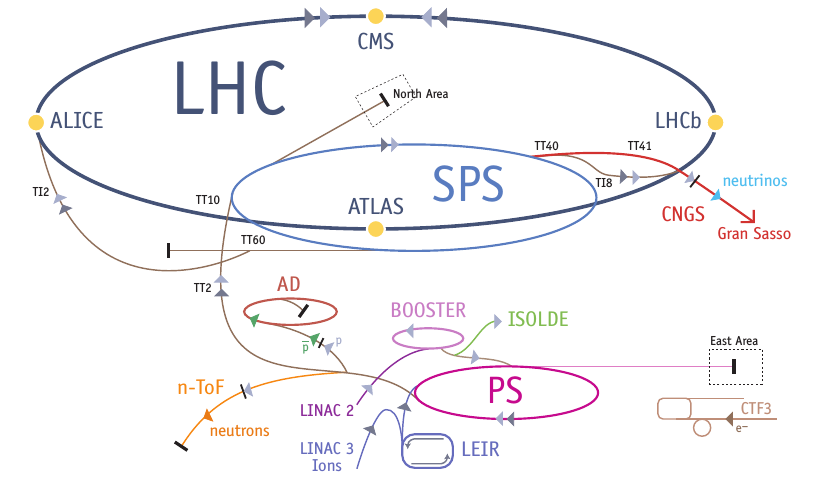
\includegraphics[width=6in]{THESISPLOTS/The_LHC.png}}
\captionof{figure}{Schematic diagram showing the full Large hadron Collider.} %Image taken from \cite{LHCB}}
\label{fig:LHC}
\end{center}
\subsection{Colliding Energy}
Protons which are hydrogen ions from hydrogen gas where the orbiting electron has been striped away are inserted into a linear accelerator called LINAC 2.
Using the electromagnetic fields in Radio Frequency~(RF) cavities, these protons are accelerated to an energy of 50\MeV creating a stream of particles called \textit{proton beams} which are arranged in packets known as \textit{bunches}. The proton beams from the LINAC 2 are injected into the circular \textit{Proton Synchrotron Booster}~(PSB) where they gain acceleration as the pass many times through the RF cavities with their energy increasing after each pass. The PSB accelerates the protons up to 1.4\GeV and injects them into the \textit{Proton Synchrotron}~(PS) which increases their energy to 25\GeV. These protons, traveling at 99.93\% the speed of light at this stage, are sent to the \textit{Super Proton Synchrotron}~(SPS) and further accelerated to an energy of 450\GeV. The 450\GeV protons are finally transferred into the LHC ring~(split into two beams accelerating in a clockwise and anti-clockwise direction) where they are accelerated for about 20 minutes to their nominal energy of 7\TeV. By now the protons are traveling with the speed of 99.9999\% the speed of light and powerful bending magnets are used to keep the beams traveling in the circular LHC ring.
\newline
In a circular particle collider like the LHC, the energy available to make new particles, which is the \textit{center of mass}~(COM) energy, denoted by $\sqrt{S}$, is simply the sum of the energy of the two beams \ie $\sqrt{S} = \mathit{E}_{\mbox{beam1}} + \mathit{E}_{\mbox{beam2}}$. This is larger than that for fixed target colliders which is $\sqrt{\mathit{E}_{\mbox{beam}}}$, and makes circular colliders favorable for producing new particles with high enough mass. For example, in the LHC, each beam is designed to have an energy of 7\TeV  making $\sqrt{S} = 14$\TeV.

%%%%%%%%%%%%%%%%%%%%%%%%%%%%%%%%%%%%%%%%%%%%%%%%%%%%%%%%%%%%%%%%%%%%%%%%%%%%%%%%%%%%%%%%%%%%%%%%%%%%%%%%%
\subsection{Luminosity}
%%%%%%%%%%%%%%%%%%%%%%%%%%%%%%%%%%%%%%%%%%%%%%%%%%%%%%%%%%%%%%%%%%%%%%%%%%%%%%%%%%%%%%%%%%%%%%%%%%%%%%%
In colliding beam experiments, the center of mass energy available for producing a new phenomenon is very important. However, the number of useful interactions producing the new phenomenon~(event) is equally important, especially in cases where the probability~(or cross section) of producing events from a rare phenomenon or physics process is very small. The \textit{Luminosity}~($\mathscr{L}$) of the  colliding beams measures the potential of a particle accelerator to produce events from a required number of interactions and serves as the proportionality factor between the number of events per second and the cross section. The luminosity can be  defined as a measure of the number of collisions that can be produced in a collider per squared area per second.  It depends on factors ranging from the flux \ie number of particles per second  of the beams, the  size of the beam  at collision and the frequency of collision. For physics experiments, the integrated luminosity which is the total luminosity over a given period of time, usually a year, gives the amount of data that has been recorded by a given detector and represents events produced from many different physics processes. From the  measured luminosity~($\mathscr{L}$) and the predicted cross section~($\sigma_{p}$) of a given physics process, we can estimate the number of events per second~(event rate~($\mathsf{R}$)) we expect to be produced in $pp$ collisions as
\begin{equation}
\mathsf{R} = \mathscr{L} \cdot \sigma_{p}.
\end{equation}
However, in measurement experiments, the observed number of events~($N$) and the measured integrated luminosity can be used to measure the cross section~($\sigma$) of a physics process using the relation 
\begin{equation}
\sigma = \frac{N}{\mathscr{A}\times\epsilon\times\mathscr{L}}, 
\end{equation}
where $\epsilon$, and $\mathscr{A}$, are the efficiency and acceptance in counting the observed number of events, respectively. This measured cross section can be compared to predictions of a model.
\par
The LHC was designed to collide proton beams with a peak instantaneous luminosity of $1 \times 10^{34}\cm^{-2}s^{-1}$ and the total integrated luminosity measured by the CMS detector is separated into the "recorded" and "delivered" integrated luminosity. Delivered luminosity refers to the luminosity delivered by LHC to CMS and one would expect this to be equal to  the amount recorded. However, there are instances when the CMS detector is unable to record data either because CMS Trigger and Data Acquisition System~(TriDAS) is down or one of the CMS sub-detectors is temporarily being repaired. Figure \ref{fig:cmslumi} shows a monthly total integrated luminosity delivered by LHC and recorded using the CMS detector during the $8$\TeV $pp$ collision.
 
\vspace{5mm}
\begin{minipage}{0.90\linewidth}
\begin{center}
\mbox{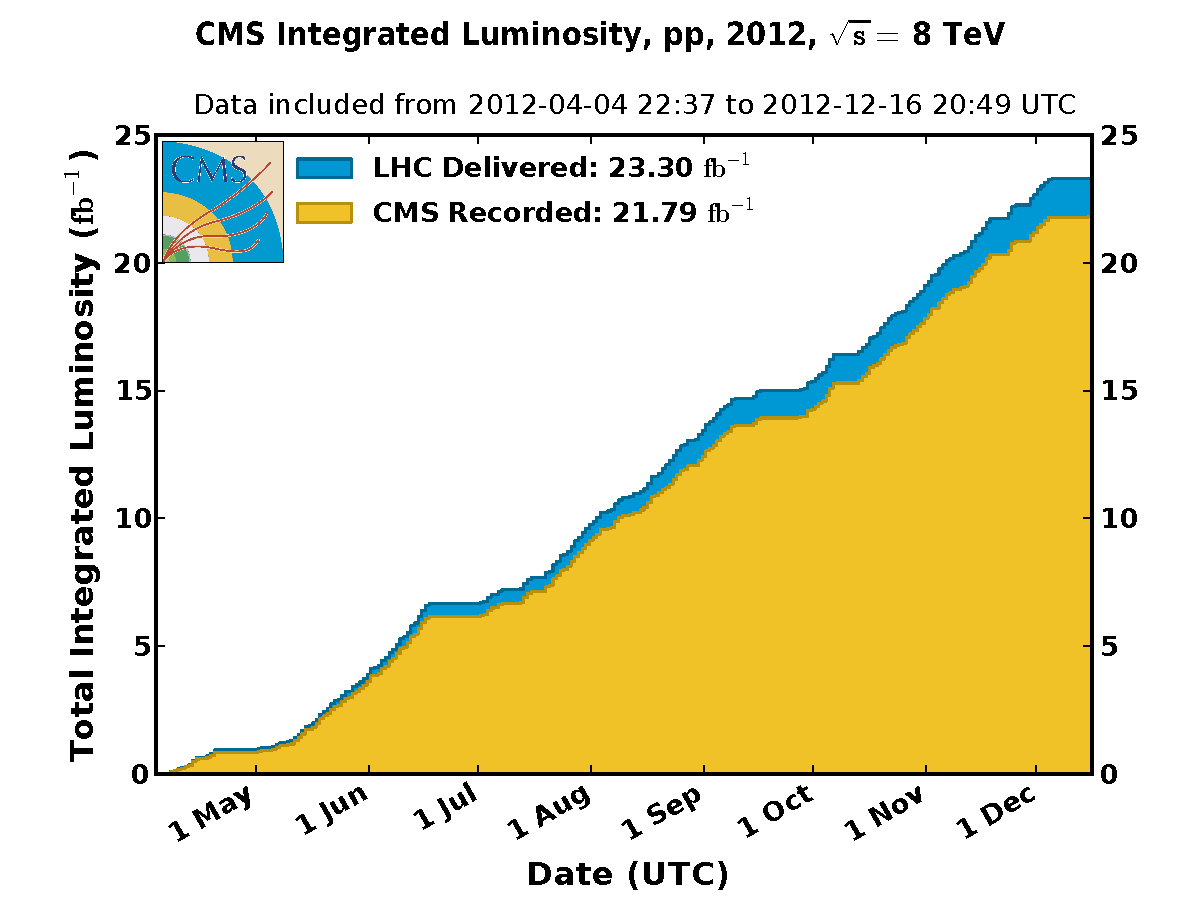
\includegraphics[scale=0.5]{THESISPLOTS/int_lumi_per_day_cumulative_pp_2012.pdf}
}
\captionof{figure}{Cumulative luminosity versus month delivered to (blue), and recorded by CMS (orange) during stable beams of for $pp$ collisions at $\sqrt{S} = 8\TeV$ in 2012.}
\label{fig:cmslumi}
\end{center}
\end{minipage}

\subsection{LHC Bunch Structure}\label{Ghost}
Of the 3564 \textit{bunch} places in an LHC orbit, only 2808 bunch places are occupied with protons. Each proton bunch has been placed inside an RF bucket during the proton beam filling process. The filling scheme is organized such that not all the RF buckets have protons. The empty buckets or beam gaps are necessary to avoid parasitic collisions near the collision point and to make room for beam halo removal and beam dump during beam cleaning, prior to and after collision.
Each RF bucket, filled or empty, is separated in time from the next one by approximately $2.5$~ns and carries about $10^{11}$ protons. During the filling in LINAC 2 and the splitting into proton bunches with each bunch occupying an RF bucket in the PS, it is possible that some empty RF buckets are also filled although they carry a much smaller proton population compared to the main proton bunch. These bunches carrying few protons can either be trailing the main proton bunch by a time of $\Delta t$ = 2.5, 5.0, 7.5, $\ldots$~ns, or leading the main proton bunch by $\Delta t$ = -2.5, -5.0, -7.5, $\ldots$~ns. If the bunch is $2.5$ to $3.0$~ns separated in time from the main proton bunch or another, it is called a \textit{satellite} bunch and if the separation is about $5.0$~ns, it is referred to as an \textit{ghost} bunch.  In Figure \ref{fig:LDM-Ghost}, we present a longitudinal profile of a typical LHC orbit showing the ghost, satellite and main proton bunches \cite{LDM}.
\par 
The presence of ghost/satellite bunches increase the uncertainty in LHC luminosity measurements and can also generate $pp$ interactions near the collision point. Effects from ghost/satellite bunches on instantaneous luminosity measurements and recorded events have been studied  by CMS, ATLAS and ALICE experiments. The results, seen in Figure \ref{fig:CMS-ATLAS-Ghost}, show a clear presence of events produced from ghost and satellite bunch collisions. CMS used the energy deposits in the endcap calorimeters to observe time spaced clusters which are consistent with expectations from ghost/satellite bunches while ATLAS uses the Longitudinal Density Monitor~(LDM) detector to study ghost/satellite bunches. The details of these studies can be found in \cite{ATLAS-GHOST, CMS-GHOST}.
\par
We summarize in Table \ref{tab:tableLHC}, the LHC design and operation conditions during LHC RUN 1. 
 
\vspace{5mm}
\begin{minipage}{0.90\linewidth}
\begin{center}
\mbox{
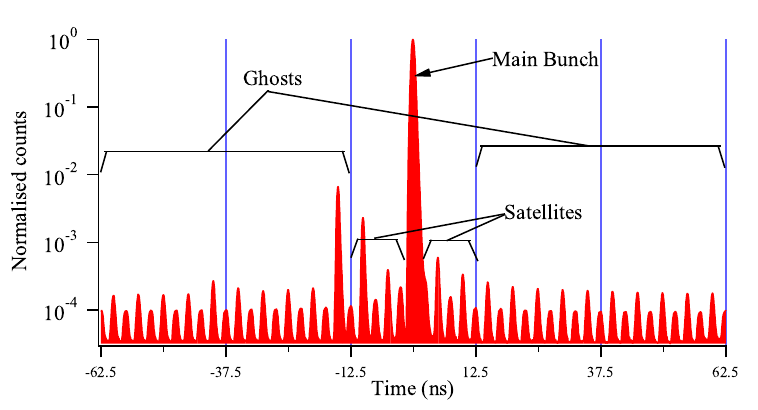
\includegraphics[height=0.5\textwidth, width=0.85\textwidth]{THESISPLOTS/Ghost-Satellite-Bunches-LDM.png}} 
\captionof{figure}{Longitudinal profile of a typical LHC proton beam taken with the Longitudinal Density Monitor~(LDM) detector. Ghost/Satellite bunches and the main proton bunch shown.}
\label{fig:LDM-Ghost}
\end{center}
\end{minipage}

\vspace{5mm}
\begin{minipage}{0.90\linewidth}
\begin{center}
\mbox{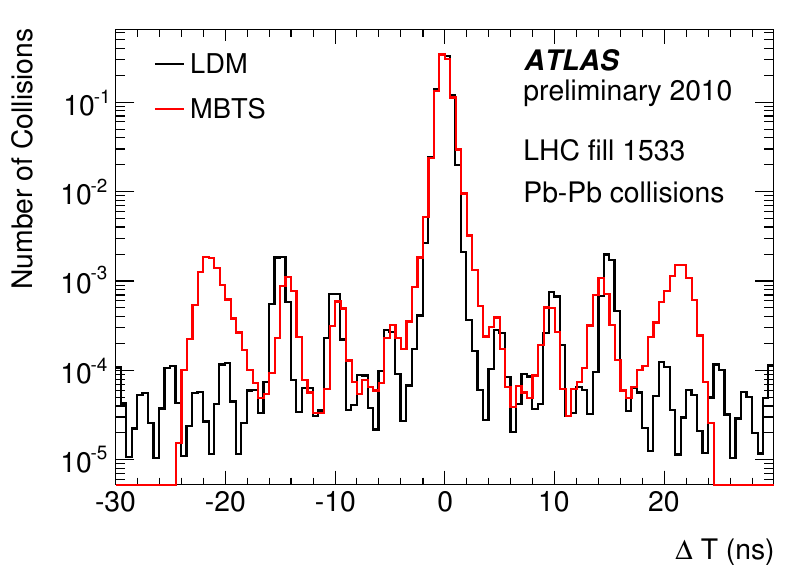
\includegraphics[height=0.5\textwidth, width=0.30\textwidth]{THESISPLOTS/ATLAS-LDM-GHOST.png} \quad
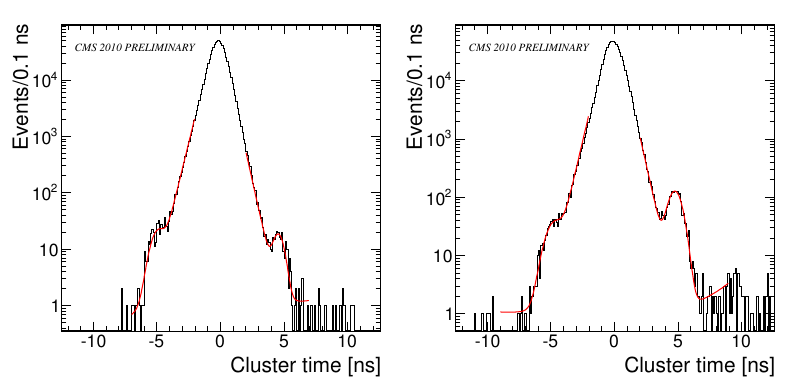
\includegraphics[height=0.5\textwidth, width=0.60\textwidth]{THESISPLOTS/CMS-Ghost-Profile.png}} 
\captionof{figure}{Left: Arrival time~(red) of events in ATLAS for LHC fill 1533 during 2010 $PbPb$ collision and an LDM profile~(black) for Beam2~(same for Beam1). Right: Cluster time in the CMS endcap calorimeters from fill 1089 of the positive endcap detector(left side of IP $z> 0$)~(left) and negative endcap detector(right side of IP, $z<0$)~(right). Both plots show a clear presence of events from Ghost/Satellite bunches with the expected time separation.}
\label{fig:CMS-ATLAS-Ghost}
\end{center}
\end{minipage}

\vspace{5mm}

\afterpage{ %
    \clearpage% Flush earlier floats (otherwise order might not be correct)
   %% \thispagestyle{empty}% empty page style (?)
  \begin{landscape}% Landscape page
   \begin{center}
  % \begin{table}[H]
   % \begin{turn}{90}
 %\setlength{\abovecaptionskip}{0pt}
  %\setlength{\belowcaptionskip}{10pt}
 % \topcaption{GMSB,GGM Phenomenology and Relevant final states}
 %\rotatebox{90}{%
  \begin{tabular}{l|l|l|l|l}
  %\hline \hline
  \multicolumn{5}{c}{\bfseries{LHC Operation Parameters 2010-2013}} \\
  \hline
  \toprule
  \bfseries{Parameter} & \bfseries{2010 value} & \bfseries{2011 Value} & \bfseries{2012/13 Value} & \bfseries{Design Value} \\
   \hline \hline
   Beam energy[Te] & 3.5  & 3.5  & 4.0  & 7 \\ 
  \hline
  $\beta^{\ast}$ in IP 5[m] & 3.5 & 1.0 & 0.6  & 0.55 \\
  \hline
   Bunch spacing [ns]& 150 & 75/50 & 50 & 25 \\
  \hline
  Number of bunches & 368 & 1380 & 1380 & 2808 \\
  \hline
  Protons/bunch  & $1.2 \times 10^{11}$ & $1.45 \times 10^{11}$ &  $1.7 \times 10^{11}$& $1.15 \times 10^{11}$ \\
  \hline
  Normalised emittance[mm.rad] & $\approx 2.0$ & $\approx 2.4$ & $\approx 2.5$ &  3.75\\
  \hline
  Peak luminosity[$cm^{-2}s^{-1}$]& $2.1 \times 10^{32}$ & $3.7 \times 10^{33}$ & $6.8 \times 10^{33}$ & $1 \times 10^{34}$ \\
  \hline
  Evts/bunch crossing & 4 & 17 & 37 &  19 \\
  \hline
  Stored Beam energy(MJ)& $\approx 28$ &  $\approx 110$  & $\approx 140$  & $\approx 362$ \\
  \hline
  Int. Luminosity by CMS[$pb^{-1}$]&  &  &  &  \_ \\
 \hline
 Circumference[km]  &26.659 & 26.659 & 26.659 & 26.659 \\
 \hline
 Dipole Magnet B[T] & 8.33 & 8.33 & 8.33 & 8.33 \\
 \hline  
  \bottomrule
  \end{tabular}
  \captionof{table}{LHC operation parameter conditions during RUN 1, 2010-2013}
  \label{tab:tableLHC}
 %\end{sidewaystable}
 %\end{turn}
 %\end{table}
 \end{center}
 \end{landscape}
 \clearpage% Flush page
}
%\lipsum % Text after
%\clearpage

\section{Compact Muon Solenoid}
\subsection{Overview}
The Compact Muon Solenoid~(CMS) detector is located at Point 5 which is one of the $pp$ collision points along the LHC ring. Its choice of design balances cost and robustness in the detection of many different particles. The detector has a simple cylindrical structure consisting of a barrel and  two endcap detectors. It also has an extensive forward calorimetry detector providing an almost $4\pi$ solid angle coverage which assures good hermetic particle detection. The overall length of 21.6\m, a diameter of 14.6\m and weight of 12,500 tons define the size of the CMS detector. Figure \ref{fig:CMS-DET} shows the CMS detector with its different sub-detectors and the type of material used in the construction.
\par 
The main feature of the CMS detector is the presence of a superconducting solenoid magnet of 6\m internal diameter. The magnet provides a strong magnetic field of $3.8$~T which causes the bending of the tracks of charge particles as they travel across the detector. The  particle's momentum is measured from the reconstructed track. 
\newline
The magnetic field encloses an entirely silicon pixel and strip tracker detector which are used for vertex finding and reconstructing the tracks of charged particles, a lead-tungstate~(\pb) scintillating-crystal Electromagnetic Calorimeter (ECAL) and a brass and plastic scintillator sampling Hadron Calorimeter (HCAL). Very long lived particles like muons are detected using gas-ionization detectors embedded in the flux-return iron-yoke located at the outermost region of the detector called Muon Chambers.
\par 
The CMS experiment uses a coordinate system with the origin coinciding with the center of the detector where the $pp$ or nominal collisions occur. This point is commonly referred to as the \textit{interaction point}~(IP). The directions of $x,y,$ and $z$-axes are as shown in Figure \ref{fig:CMSDCORD}. However, for particle identification, CMS uses a more convenient coordinate system based on the polar coordinates where the azimuthal angle, $\phi$, is measured in the $x-y$ plane, with $\phi = 0$, being the $x$-axis and $\phi = \pi/2 $, the $y$-axis. The radial distance in this plane is denoted $R$, and the polar angle $\theta$, measured from the $z$-axis is related to \textit{pseudo-rapidity}, $\eta$, through the relation: $\boldmath{\eta = -\ln \tan(\frac{\theta} {2})}$. 
The coordinate system $(\eta, \phi)$, and its radial distance $R$, identifies a point in the cylindrical volume of the CMS detector. We will now describe the CMS subdetectors used in our analysis.
%\clearpage
\begin{center}
\centering
\mbox{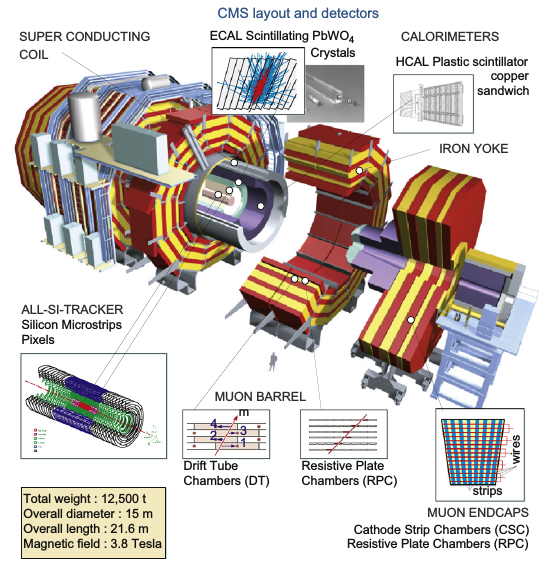
\includegraphics[width=10cm]{THESISPLOTS/CMS_LAYOUT_AND_DETECTORS.png}} 
\captionof{figure}{CMS Detector showing the different subdetectors and their material.}
\label{fig:CMS-DET}
\end{center}

\begin{center}
\centering
\mbox{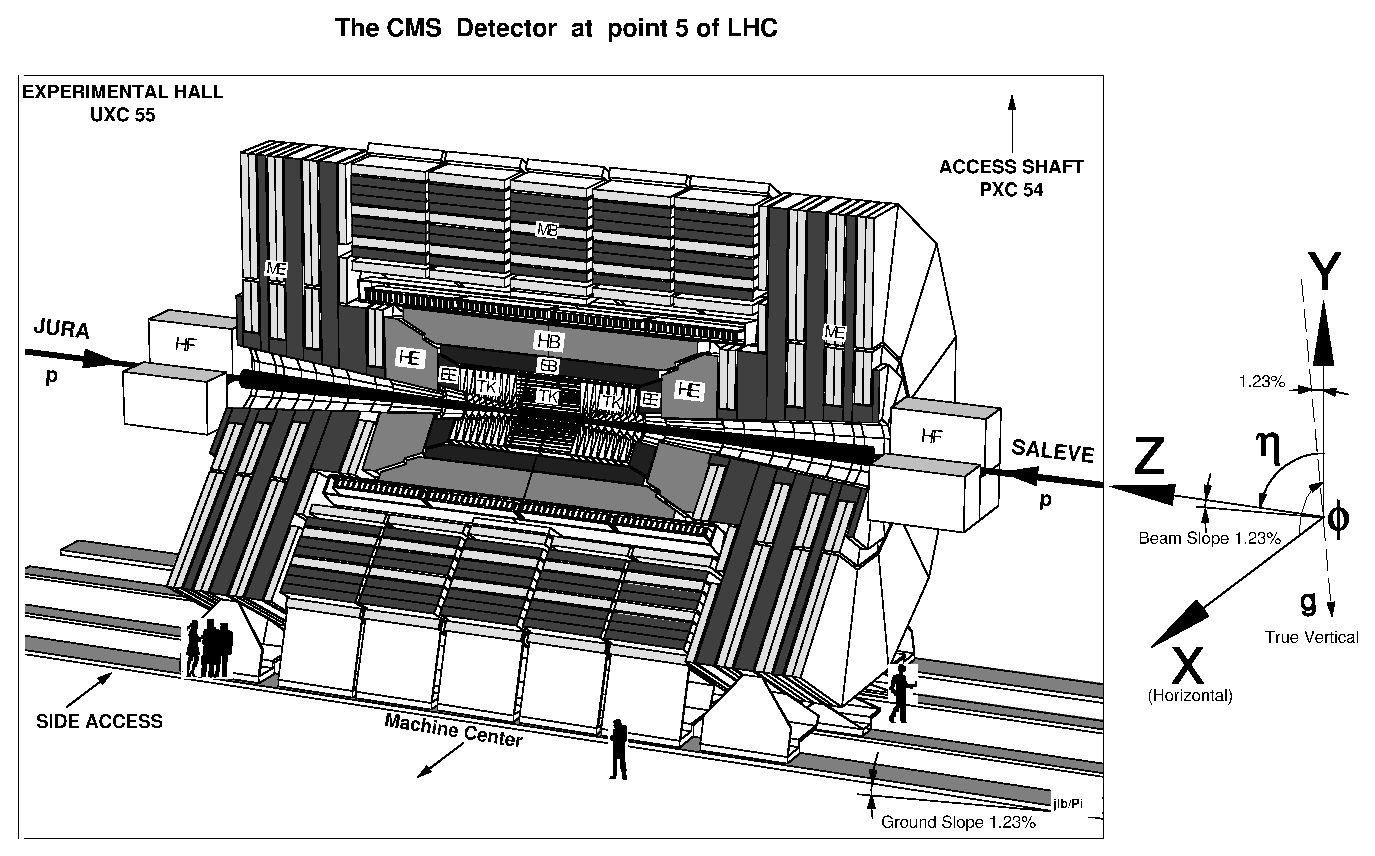
\includegraphics[scale=0.5]{THESISPLOTS/CMS_DETECTOR.eps}} 
\captionof{figure}{CMS detector schematic view with definition of $x-y-z$ coordinates.}
\label{fig:CMSDCORD}
\end{center}

\subsection{Calorimeters}
The calorimeter absorbs a good fraction of energy of an incident particle and produces a signal with an amplitude proportional to the absorbed energy. The energy absorption happens through the cascade production of secondary particles with the energy of the incident particle directly proportional to the number of secondary particles produced. The are two types of calorimetry choices used in the CMS detector: the \textit{Electromagnetic Calorimeter}~(ECAL) which is used for absorbing the energy of electromagnetic particles like photons and electrons and a \textit{Hadronic Calorimeter}~(HCAL) constructed with more than one type of material and is used for stopping and absorbing the energy of hadrons such as kaons and pions through strong interactions. The combined calorimeter subdetectors in CMS covers a region in $|\eta| < 5$, making it nearly hermetic which is needed for good missing transverse energy measurements. The ECAL and HCAL are arranged in a nested fashion shown in Figure \ref{fig:ECAL-HCAL} with the HCAL enclosing the ECAL so that electromagnetic particles can be distinguished from hadronic particles by comparing the depth of the particle shower penetration in both calorimeters.

\begin{center}
\centering
\mbox{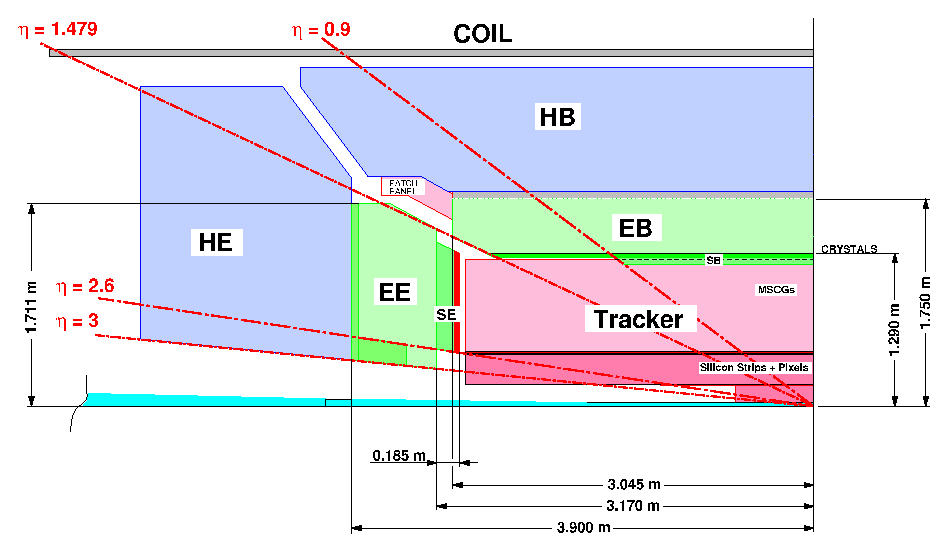
\includegraphics[scale=0.5]{THESISPLOTS/ECAL-HCAL.eps}} 
\captionof{figure}{Schematic diagram of CMS calorimetry system with HCAL enclosing ECAL in the barrel and endcap regions.}
\label{fig:ECAL-HCAL}
\end{center}
%Low energy electrons loss their energy through elastic scattering and annihilation while
\subsubsection{Electromagnetic Calorimeter}
 The Electromagnetic Calorimeter~(ECAL) detects photons and electrons through their interaction with the atoms of the lead tungstate~(\pb) crystals. During this interaction process which might happen through Coulomb scattering~(electron-neutron scattering), Compton scattering~(photon-electron scattering), photon emission~(also known as \emph{Bremsstrahlung}) and \emph{electron-positron pair production}, the incoming photon or electron deposits practically almost all of its energy into the detecting medium. Electrons loss most of their energy, due to their small mass, through radiation~(photon emission). High energy electrons and photons of several \GeV deposit their energy to the \pb crystals through Bremsstrahlung and pair production processes producing electrons, positrons and photons in the process which subsequently produce more electrons, positrons and photons creating an avalanche of electrons, positrons and photons known as an \textit{electromagnetic showers}. The process stops when the electron or photon energy becomes low. The probability of an electromagnetic particle with high energy to interact either through Bremsstrahlung or pair production with the detecting material is proportional to the nuclear charge, \text{Z}, of the material.
\par 
The choice of \pb crystals as the calorimetry material by CMS for operation in the LHC environment is because of the following reasons: \pb crystal is a high \text{Z} material with a density of 8.28~g/$\cm^{3}$), has a short radiation length~($X_{0}$=0.89\cm) and a small Moli$\grave{e}$re radius~(22\cm). The dense nature of the \pb crystals allow for the electromagnetic shower to develop early and therefore likely to be fully contained within a compact detector like CMS. The short radiation length ensures that on average about $95$\,\% of the electromagnetic shower energy produced by the photon or electron is contained within a crystal volume of about 9 crystals while the small Moli$\grave{e}$re radius reduces the transverse spread of the electromagnetic cascade from multiple scattering of electrons and helps improve the estimation of the transverse position of impact of an incident particle. The arrangement of the \pb crystals also provide a fine granularity for measuring the particle's energy by providing fewer overlap of particle signals.
\newline
\pb crystal is also preferred to other crystal materials because of its high radiation resistance and fast scintillation decay time which is comparable to the LHC bunch crossing interval of 25~ns required for the high radiation dose and fast timing~(25~ns proton bunch spacing) LHC environment.  About 80\% of the energy absorbed by the \pb crystal is emitted as light in less than 25~ns.  
\par 
The ECAL has 75848 \pb crystals in total mounted in a cylindrical geometry, with a barrel~(\textsc{EB}) and an endcap~(\textsc{EE}) structure. 
\newline
The EB region of the ECAL covers a pseudo-rapidity of $\vert \eta \vert< 1.479 $. It has 61,200 crystals providing a granularity of 
$360$ degree fold in $\phi$ and $(2 \times 85)$-fold in $\eta$. The crystals are mounted in a quasi-projective geometry so that their axes make an angle of 3\% with respect to a line vector from the nominal interaction vertex in $\eta$ and $\phi$ directions. This is to avoid loss of energy into cracks aligned with a particle's trajectory. A crystal in EB is approximately $0.0174\times0.0174$ in $(\eta,\phi)$, $22\times22\mm^{2}$ at its front face and $26\times26\mm^{2}$ at its rear face. Each crystal is 230\mm long corresponding to about 25.8~$X_{0}$ radiation lengths. The crystal's radial distance measuring from the center of the face of the crystal to the beam line is 1.29\m. A number of crystals are placed in a thin-walled alveolar structure made with aluminum forming a \textit{submodule}.  
Each submodule is arranged into 4 modules of different types according to their $\eta$ position. There are about 400 to 500 crystals in each module and these 4 combined make one \textit{supermodule} containing 1700 crystals.To reduce crystal reflective lost, the aluminum surface is coated to avoid oxidation leading to coloration. On the rear end of each EB crystal, two \textit{Avalanche Photodiodes}~(APD)  is glued to collect the scintillating light from the crystals converting light into charge current which is further collected by the read-out electronics.
 \newline
The EE region covers a pseudo-rapidity region of $1.479 <\vert \eta \vert < 3.0$ with a \textit{Preshower}~(\textsc{ES}) detector made of silicon strip sensors interleaved with lead placed immediately in front of it. The purpose of the preshower is to identify photons from the decay of neutral pion, $\Ppizero \rightarrow \Pphoton\Pphoton$, and also to help separate photons producing electrons through pair production from photons not producing electrons before their arrival at the EE. 
The endcap located on the $+z$ side of the nominal interaction is denoted \textsc{EE}$+$ while the other located on the $-z$ side  is denoted as \textsc{EE}$-$. The longitudinal distance between the IP and the center of the surface of the \textsc{EE} crystal is $3.154$\m. Each endcap is divided into two halves called \textit{Dees} with each Dee holding 3662 crystals. 
Crystals in \textsc{EE} with identical shape are grouped into 5$\times$5 mechanical units called \textit{supercrystals}~(SC). 
The crystals in the SC form an $x-y$ grid. Each crystal is 220\mm~(24.7~$X_{o}$) in length and has a front and rear face cross sections of $28.62\times28.62\mm^{2}$ and $30\times30\mm^{2}$, respectively. 
A \textit{Vacuum Phototriode}~(VPT) instead of an APD is glued on the rear face of each crystal for receiving and converting the scintillating light into electrical signals. The VPT is used in the \textsc{EE} because of its high resistance to radiation and smooth operation in a strong magnetic field environment. CMS uses APDs and VPTs because they are not affected by the high magnetic field and they have a high gain relative to regular photodiodes which have no gain. Although the light yield for \pb crystals is rather low~($\approx 70$~photons/\MeV), these photo-detectors have internal gain~($50$ for APDs and 10 for VPTs) and quantum efficiency of $75$\,\% for APDs and $20$\,\% for VPTs of the emission wavelength which makes it possible for detecting signals from incident particles with energies of a few to high \GeV. The signals from the APDs and VPTs are amplified and digitized by voltage-sensitive analogue-to-digital converters and transported through optical fibres as light signals to the underground counting room which is located adjacent to the CMS experimental cavern.
\newline
The energy resolution and geometry structure of the ECAL ensures that the photon or electron's energy, arrival time, position and even the direction through the shape of its electromagnetic shower in the crystals is measured with good precision.

\vspace{5mm}
\begin{minipage}{0.99\textwidth} 
\begin{center}
\centering
\mbox{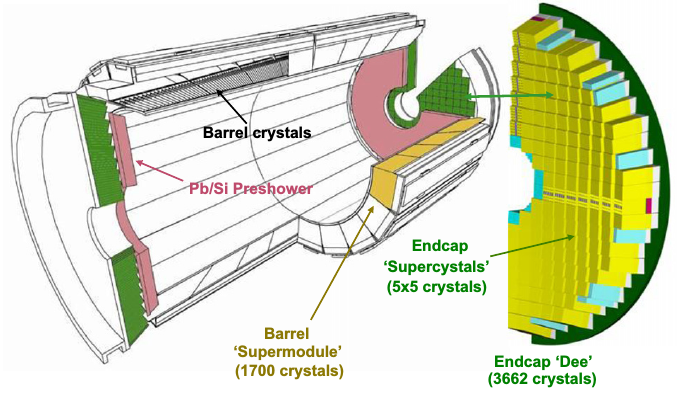
\includegraphics[height= 0.55\textwidth, width=0.8\textwidth]{THESISPLOTS/CMS-ECAL-EB-EE.png}}
%\mbox{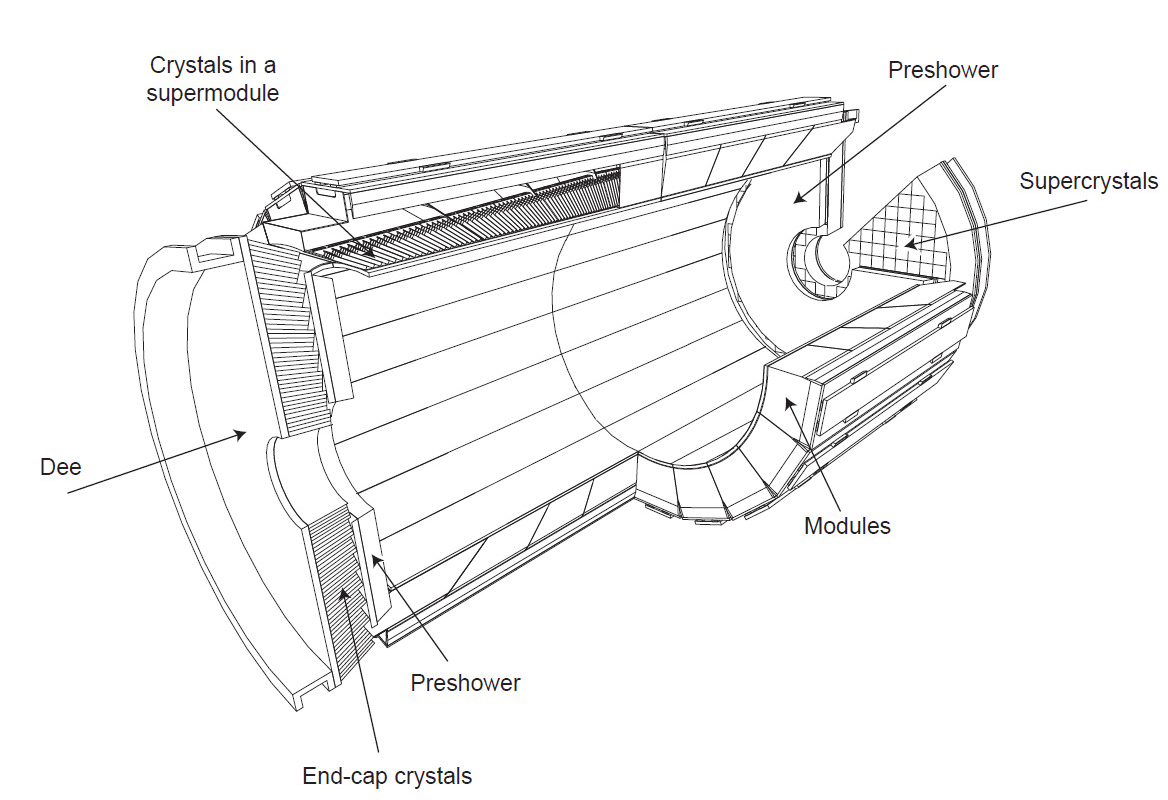
\includegraphics[scale=0.2]{THESISPLOTS/CMS-ECAL.png}}
%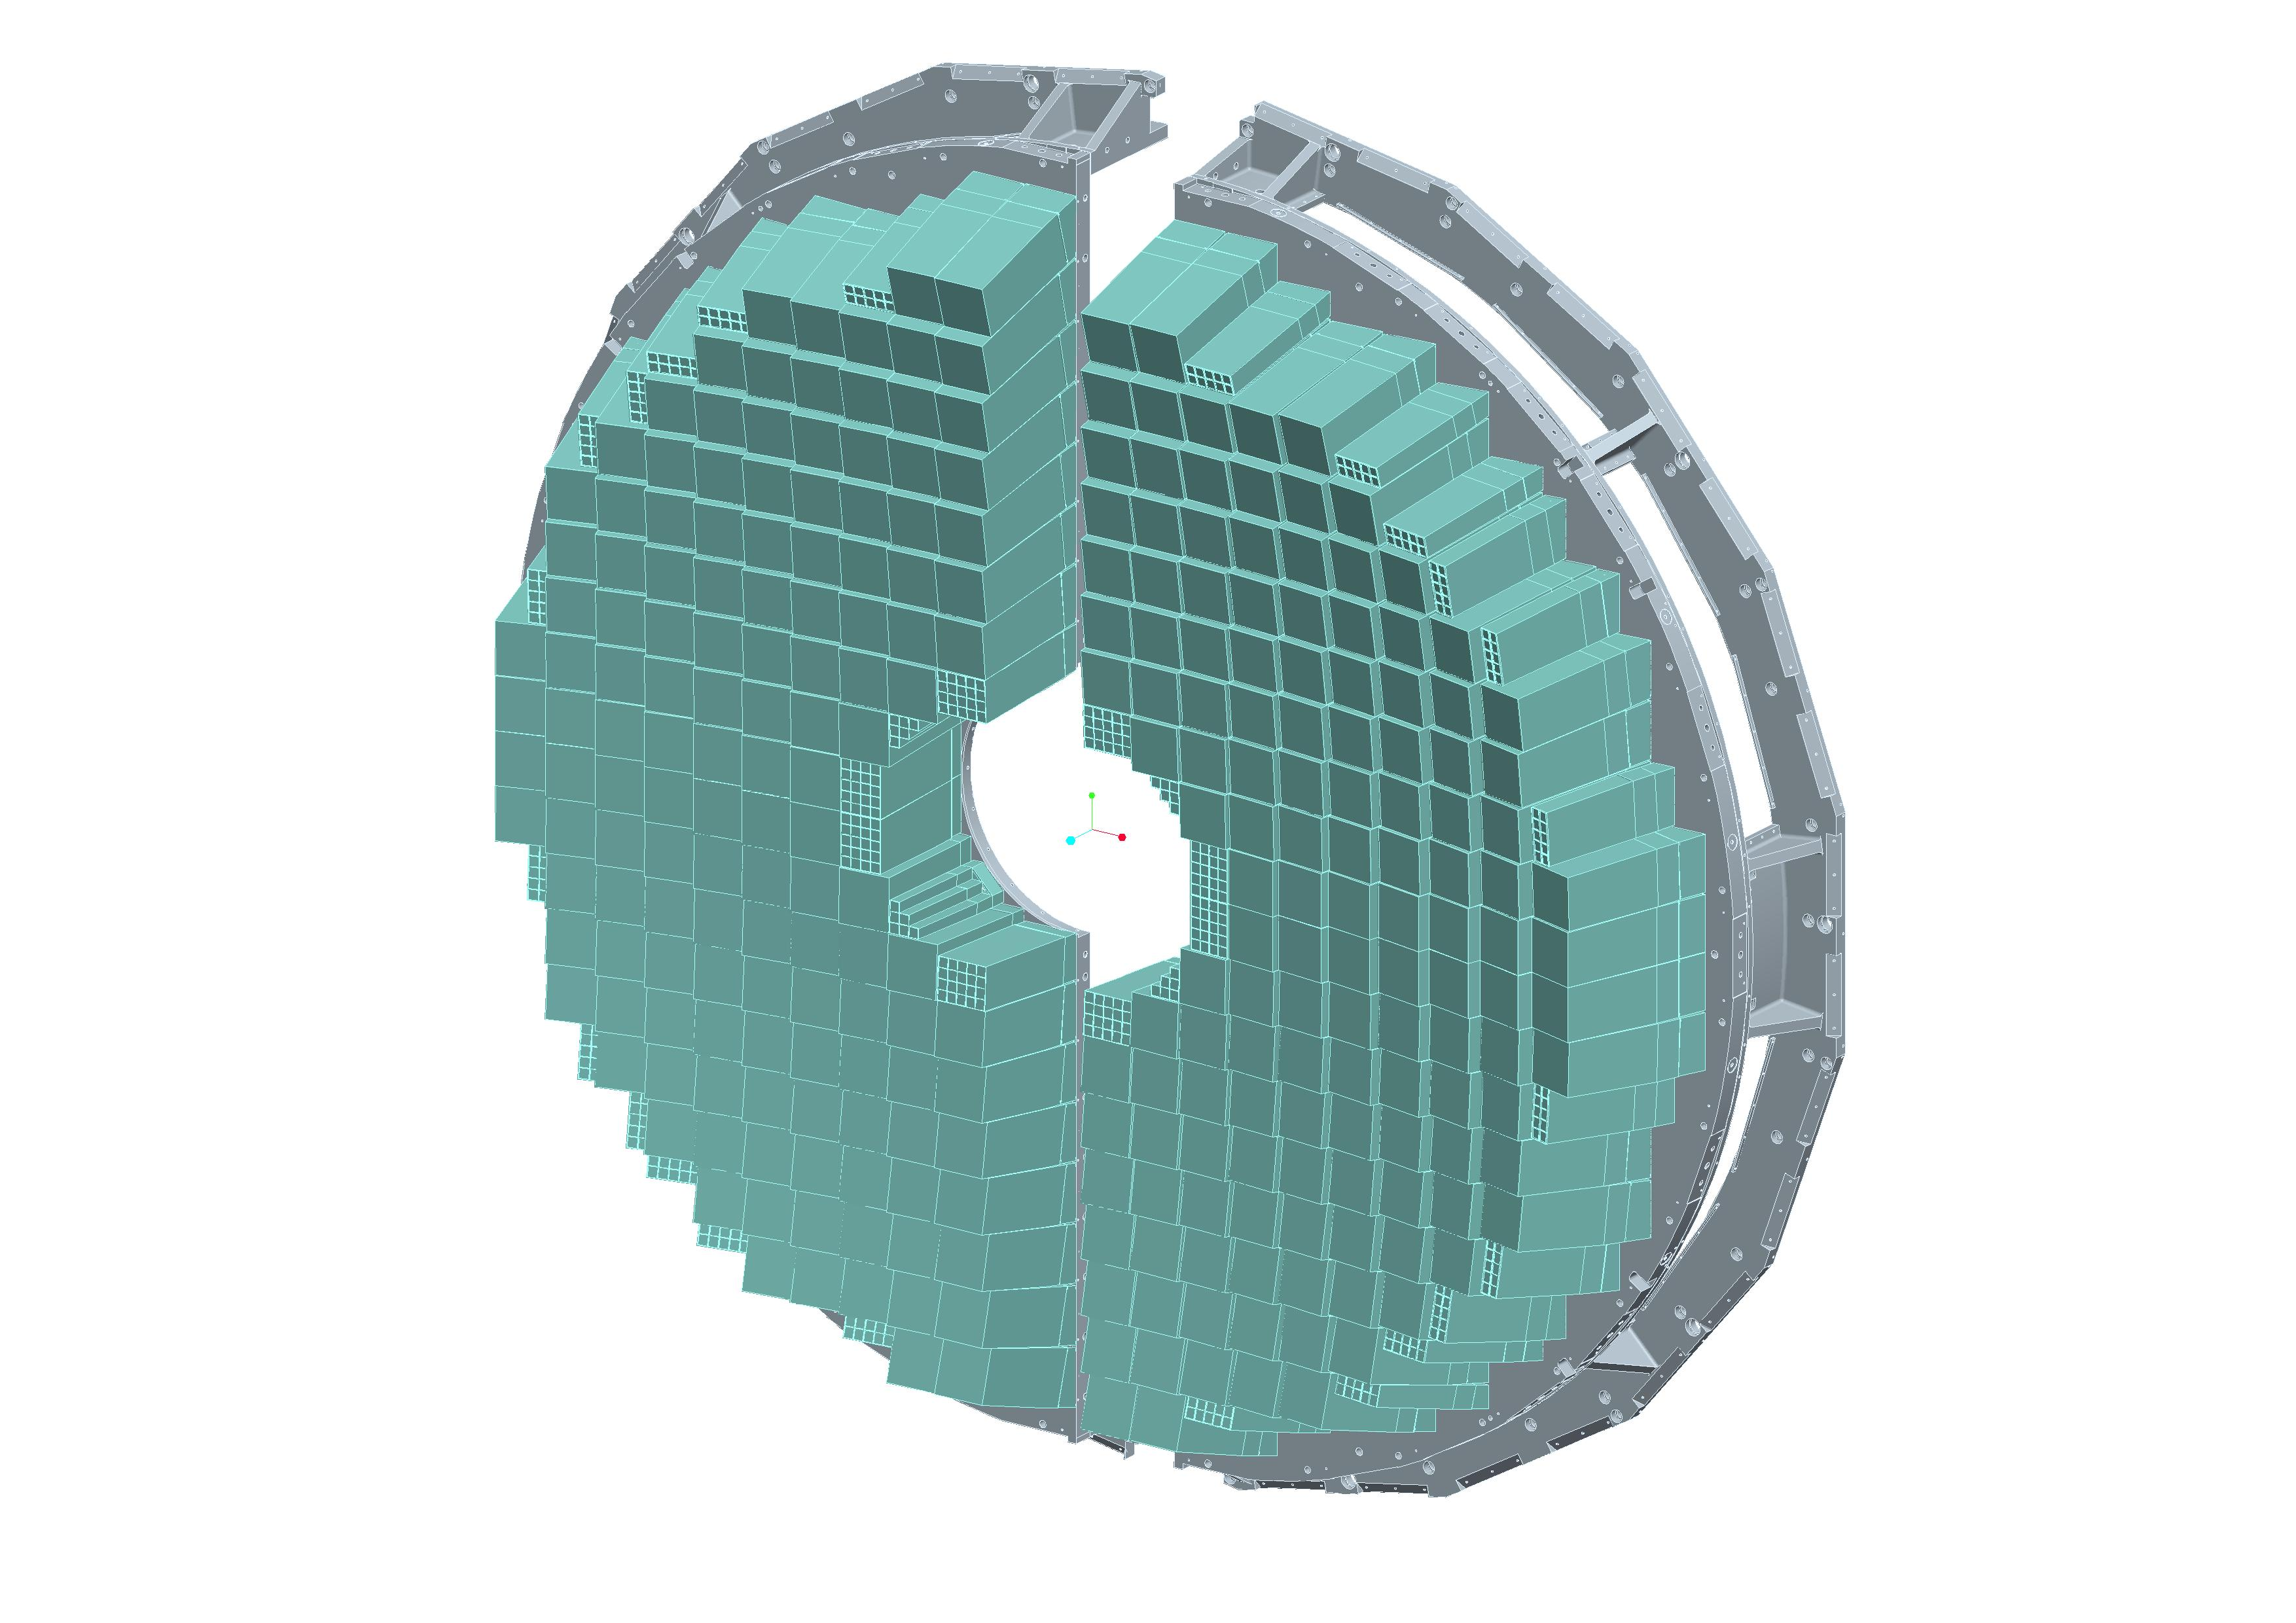
\includegraphics[scale=0.06]{THESISPLOTS/endcap_CMS.png}} 
\captionof{figure}{Layout of the CMS electromagnetic calorimeter showing the arrangement of crystal modules, supermodules in the barrel with the preshower infront of endcap with supercrystals.}
\label{fig:CMSECAL}
\end{center}
\end{minipage}


\subsubsection{ECAL Readout Electronics}\label{ecalreadout}
%%%%%%%%%%%%%%%%%%%%%%%%%%%%%%%%%%%%%%%%%%%%%%%%%%%%%%%
%The ECAL electronics readout system fully described in \cite{ECALREADOUT} is a light-to-light system.
%from each VFE is typically 1.1, 0.75, 0.6 ADC counts for gains 12, 6 and 1 respectively. This would be about 40~MeV for gain 12.
%Scintillating light from the \pb crystals is readout and converted into electric charge using Avalanche Photo-Diodes~(APD)  in EB or Vacuum Photo-Triodes~(VPT) in EE. 
%\newline
The ECAL readout electronics is divided into an On-Detector or Front End~(FE) board and an Off-Detector~(OD) electronics. The FE board is installed inside the detector volume behind the crystals and infront of the hadron calorimeter and is made with radiation-hard electronics to withstand the high radiation dose. Data from the FE is transferred by radiation hard fibres to the OD electronics which is in the underground service cavern located approximately 80\m from the CMS detector. 
\newline
A Clock and Control Unit~(CCU) chip on each FE board communicates through bi-directional optical links with the Clock and Control System~(CCS) board of the OD. These links carry clock and control  signals and the trigger Level 1 accept~(L1A) signal from the Timing, Trigger and Control~(TTC) board and the Trigger Control System~(TCS). A voltage controlled Quartz Phase-Lock Loop~(QPLL) time jitter-filter and clock multiplier chip  with an output clock jitter of 16~ps rms ensures that the LHC clock signal is transmitted to both the FE and OD electronics for synchronization.
\par
Each FE board, shown in Figure \ref{fig:readout2}, receives signals from a group of crystals typically forming a $5\times5$ crystal matrix and hosts five Very Front End~(VFE) boards with each VFE board holding five analog channels. Each channel, shown in Figure \ref{fig:readout1}, is carrying the signal from a single crystal and consists of a Multi-Gain Pre-Amplifier~(MGPA) and three identical 12 bit Analog-to-Digital Converters~(ADC), which are used to amplify, shape and digitize the signal coming from the Photo-Diode.
\newline
The MGPA chip has 3 gain ranges with gain ratios of 1, 6 and 12 to span the overall dynamic range of the signal which can go from 12\MeV up to 1.7\TeV. Equipped with a Capacitor-Resistor-Resistor-Capacitor~(CR-RC) filter with a pulse shaping time of 40~ns and less than 1\% of non-linearity, the MGPA ensures a uniform pulse shape matching and linearity across all 3 gain ranges allowing for precise pulse shape reconstruction.
\newline
The required readout and precision performance of the FE electronics demands a 12-bit ADC chip with a sampling frequency of 40~MHz to digitize the analog pulse signal of the highest unsaturated range into 10 discrete samples with an electronic noise  of about 40\MeV. The FE card stores the digitized crystal data~(ten 40~MHz discrete samples per channel) in 256-word-deep memories called \textit{pipelines}. Five such pipelines and the logic to calculated the energy sum of 5 crystals once every LHC proton bunch crossing is integrated into a $0.25~\mu\m$ technology FERNIX ASIC chip. Each VFE card is serviced by one such chip allowing for the energy to be summed in strips of 5 crystals along $\phi$. In EE the five strip energy sums are transmitted to the  Trigger Concentration Card~(TCC) on the OD electronics, while for EB, a sixth chip sums the five strip energy sums and calculates the "fine-grain" electromagnetic bit which identifies the electromagnetic shower candidates on the basis of the energy profile of the $5\times5$ crystal matrix or \textit{Trigger Tower}~(TT). The TT energy sum and the fine grain bit are transmitted to the TCC at 800~Mbits/s. The corresponding crystal data~(the ten 40~MHz discrete samples per crystal) upon receipt of a positive trigger L1A decision, is transmitted to the Data Concentration Card~(DCC) also on the OD electronics system over a distance of approximately 80\m through optical fibres at a data transfer rate of 800~Mbits/s.
\par 
  The OD electronics system, shown in Figure \ref{fig:readout}, hosts the DCC, TCC and CCS electronic boards. It serves both the Data Acquisition~(DAQ) and trigger paths.  In the DAQ path, the DCC collects the digitized crystal data from up to 68 FE boards and performs data verification and data reduction based on readout flags from the Selective Read-Out  Processor~(SRP) system, while in the trigger path, the TCC collects trigger data from up to 68 FE boards corresponding to a supermodule in the barrel and 48 FE boards  corresponding to the inner and outer  part of a $20^{o}$ in $\phi$. The TCC completes a Trigger Primitive Generation~(TPG) process started at the FE by computing \textit{trigger primitives} and synchronized them by the Synchronization and Link mezzanine Board~(SLB) before  their eventual transmission to the Regional Calorimeter Trigger system at each LHC proton bunch crossing. Each Trigger Primitive~(TP) consist of the summed transverse energy deposited in each TT and the fine-grain bit. The 24 bits TPs are stored in the TCC during a Level-1 trigger latency and multiplexed into an 8-bit word encoding the summed transverse energy in a tower and the fine-grain bit and finally transferred to the DCC at a rate of 1 word/25~ns.
\par 
The CCS is tasked primarily with distributing fast timing signals~(LHC 40.08~MHz clock, L1A  and control signals to the TCC, DCC and CCUs of the FE board. By interfacing the on- and off-detector electronics to the TCS and Trigger Throttling System~(TTS), the CCS synchronizes all the activities of the OD and configures the on-detector electronics \cite{ECALREADOUT}.  
\newline
The 40.08~MHz LHC Bunch-Crossing~(BX) clock and 11.246~KHz~(88.9\mus) orbit signals from the RF generators of the LHC machine are broadcast over singlemode optical fibres from high power laser transmitters at the Prevessin Control Room~(PCR) to the four LHC experiments. The combined signals  are received at CMS by a TTC machine interface~(TTCmi) minicrate carrying an LHC clock receiver~(LHCrx) module and a TTC Clock fanout~(TTCcf) module. Embedded in the TTCmi is a voltage controlled \textit{Quartz Phase-Lock Loop}~(QPLL) ASIC with a clock frequency or locking range of 40.0749~MHz to 40.0823~MHz. The QPLL acts as a jitter-filter and clock multiplier for clock signals operating at the LHC bunch-crossing frequency with and output clock time jitter up to 16 picoseconds~(ps) in rms. The QPLL adjusts for any clock phase and then makes multiple copies of the LHC clock signals before distributing them to the local TTC transmitters. The local TTCcf distributes the low-jitter LHC clock signals to the TTC receiver~(TTCrx) module of the TTC system which is eventually distributed through optical fibres to FE boards, trigger and OD readout electronics used for Level trigger accept, bunch counter reset, bunch crossing number event counter reset and event number and the millions of electronics channels. The TTCmi also has master phase adjustment for the  orbit signal and facilitates monitoring of clock signal quality. The local TTC system is programmed to distribute to all the trigger synchronization circuits or Synchronization and Link mezzanine Board~(SLB) the  Bunch-Crossing zero~(BC0) broadcast signal. 
\newline
In the SLB of each TCC, the BC0 timing is synchronized \cite{TRIGSYNC} to match the arrival of the bunch zero or first bunch crossing TP data at the SLB. The synchronization circuits make use of FIFOs to archive the synchronization \ie after a clear FIFO is executed during the LHC extraction gap of 127 missing proton bunches of the LHC orbit, the first data entering each FIFO must correspond to the bunch zero crossing. This synchronization is needed to account for the non-negligible and unpredictable phase on the trigger primitives arrival time to the processors introduced by different particle flight paths to different regions of the detector, different optical transmission fibre lengths and different phase lock delays in the electronic serializers and ensures that the electromagnetic and hadronic calorimeter trigger primitives in each TT is time aligned with respect to the "bunch 0 clock" which corresponds to the start of the LHC orbit. The synchronized trigger primitives are sent at 1.2~Gbits/s to the Regional Calorimeter Trigger through 10\m electrical cables where with HCAL trigger primitives, the electron/photon and jet candidates are computer together with their total transverse energy. 
\newline
In the DCC the data integrity is verified and formatted together with the TCC information, the selective readout flags and the crystal data of the selected TT according to the selective readout processor flags. Words of 64 bits are formed and sent to the DAQ at L1A rate provided by the trigger system.
% In the DCC it is stored in a pipeline buffer until a Trigger Level 1~(LV1) accept decision is received after which it is sent to the DAQ. The digitized data in the TCC is used for completion of the Trigger Primitive Generation~(TPG) started at the FE and and eventual transfer to the LV1 trigger system.  The TPs are sent to the Trigger Concentration Card~(TCC) on the OD electronics at a rate of .

\vspace{5mm}

\begin{minipage}{0.99\textwidth} 
\begin{center}
\mbox{
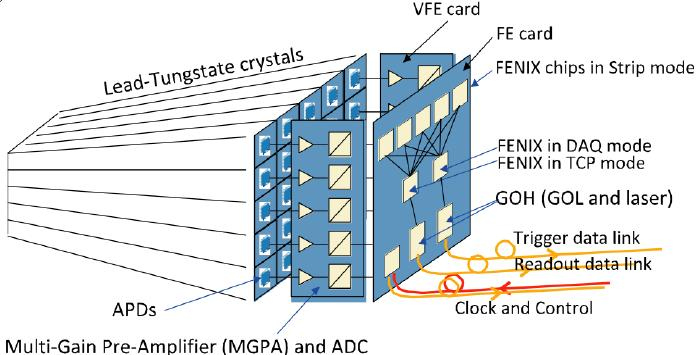
\includegraphics[height=0.6\textwidth, width=0.9\textwidth]{THESISPLOTS/ECAL-FRONT-END-ELECTRONICS.jpg}
%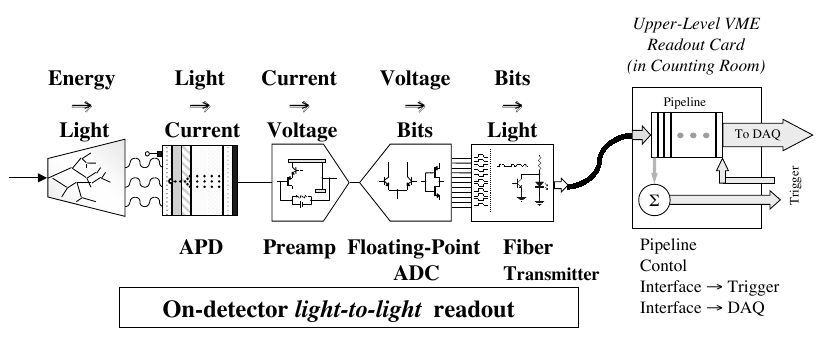
\includegraphics[height=0.5\textwidth, width=0.50\textwidth]{THESISPLOTS/CMS-ECAL-READOUT-CHAIN.png} \quad
} 
\captionof{figure}{Schematic diagram of the ECAL electronics readout  Trigger Tower~(TT) or Front End~(FE) board.}
\label{fig:readout2}
\end{center}
\end{minipage}


\vspace{5mm}
\begin{minipage}{0.99\textwidth} 
\begin{center}
\mbox{
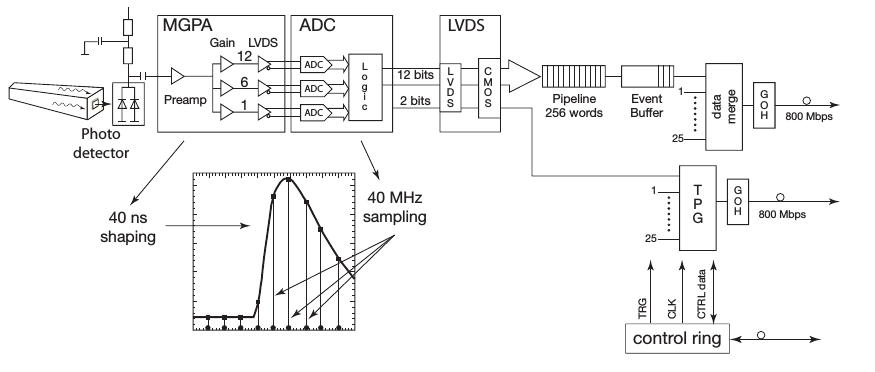
\includegraphics[height=0.6\textwidth, width=0.9\textwidth]{THESISPLOTS/ReadOut.png}
}
\captionof{figure}{Schematic diagram of the ECAL electronics readout for a single crystal.}
\label{fig:readout1}
\end{center}
\end{minipage}


\vspace{5mm}
\begin{minipage}{0.99\textwidth} 
\begin{center}
\mbox{
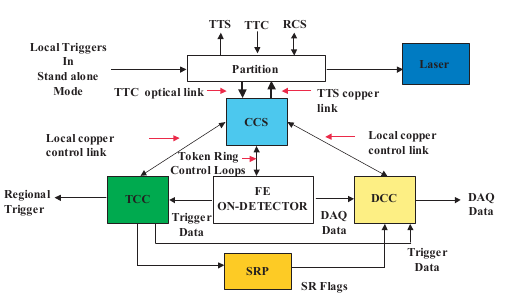
\includegraphics[height=0.6\textwidth, width=0.9\textwidth]{THESISPLOTS/ECAL-Off-Detector-and-ReadOut-Electronics.png}
}
\captionof{figure}{Schematic diagram of the ECAL Off-Detector and Readout Architecture.}
\label{fig:readout}
\end{center}
\end{minipage}



%Photodiodes like APDs and VPTs are similar to silicon photodiodes, with the exception that they have a buried p-n junction reversed-biased at a very high electric field. The photo electrons arriving at the junction undergo avalanche multiplication giving the device a gain.
%This homogenous design of the ECAL provides it with a performance which is optimal(by design) in its potential to discover a Higgs in the mass region 
% less than $130$\GeV/$c^{2}$ through the decay $\displaystyle{H\rightarrow\gamma\gamma}$. 
% Homogenous design implies reduced noise in the detector  thus better resolution since only a single material type is in use.
%ECAL has a current  timing resolution better than 500~ps for large energy deposits(more than 10-20~GeV in the \text{EB})~\cite{TIME} 
%and an energy resolution of ${\displaystyle\sigma/E\approx 0.45\,\%}$ for unconverted photons with energies above 100~GeV~\cite{CMSTDR}.
\subsubsection{Hadronic Calorimeter}
The Hadron Calorimeter~(HCAL) is important for the measurement of protons, pions, kaons, fragmenting quarks and gluons also known as \textit{jets} with energies in the \GeV-\TeV range and neutrinos or exotic particles producing apparent missing transverse energy. High-energy hadrons traveling through a medium transfer their energy to the constituent atoms in the medium through ionization or excitation of atoms in the medium. This energy deposition is through the formation of ion-electron pairs~(positive ion and electron) which ultimately leads to the production of \textit{hadronic showers}. A hadronic shower has an \textit{electromagnetic}~(em) and a \textit{non-electromagnetic}~(non-em) components. The em component which has one to two thirds of the energy deposited by the high-energy hadron is measured in the same way as in ECAL using an active scintillating material while the non-em shower energy is deposited in an absorber material through the inelastic collision of the incident hadron with the nucleus of the non-active absorber material and does not contribute to the measured signal but rather in the production of secondary hadrons which travel through the next layers of the absorber material producing further hadrons and very densely ionizing particles. This combination of active and non-active material is the chosen design for high-energy hadron detection in HCAL and is the reason why the HCAL is referred to as a \textit{Sampling Calorimeter}.
\par 
The HCAL is comprised of four distinct subdetectors: the Hadronic Barrel~(\text{HB}),   Endcap~(\text{HE}), Outer Barrel~(\text{HO}) and  Forward~(\text{HF}). Unlike the ECAL, the HB, HE and HO subdetectors are scintillator-sampling calorimeters using brass plates as the inactive absorber material and plastic scintillator tiles with embedded wavelength shifting fibers~(WLS) to bring out the light as the active material. The brass plate is used for absorbing and so stopping the high-energy hadron producing hadronic showers with an em~(particles like $\Ppizero$, $\Peta$ and other mesons generated in the absorption process which decay to photons and develop electromagnetic shower) and non-em~(mostly charged pions and kaons) components while the plastic scintillator with WLS is used for measuring the energy of the em component. The first active layer of the scintillating tiles is situated directly behind the ECAL in order to actively sample low energy showering particles from the support material between the ECAL and HCAL. The plastic scintilator, chosen for its long-term stability and moderate radiation hardness, is divided into $16$ $\eta$ sectors resulting in segmentation of $\Delta\eta\times\Delta\phi=0.087 \times\ 0.087$. The scintillating light is collected and brought to Hybrid Photodiodes~(HPDs) through the WLS in the HB and HE. HPDs have high electrical noise and was used during the CMS data recording of this thesis have been replaced with \textit{silicon photon multipliers}~(SiPM) which have low noise during the CMS detector upgrade in 2013-2014.
\newline 
The HB, covering the region $|\eta| < 1.3$, is divided into two-half barrel~(HB+ and HB-) sections with each composed of 18 identical $20^{o}$ wedges in $\phi$. Each wedge is made of flat brass alloy and steel~(only front and back plates) absorber plate. The HO is an extension of the HB outside the solenoid and utilizes the solenoid coil as an additional absorber. It is used to identify the starting shower and to measure the shower energy deposited after HB. For this reason the HO is also known as the \textit{tail catcher}.
The HE covers the region $1.3 < \eta < 3.1$, and has plastic scintillation tiles with granularity of  $\Delta\eta\times\Delta\phi=0.087 \times\ 0.087$ for $|\eta| < 1.6$ and  $\Delta\eta\times\Delta\phi=0.17 \times\ 0.17$ for $|\eta| > 1.6$. This granularity provides good measurement of forward moving particles through non-overlapping showers. 
\newline
The \text{HF} occupies a pseudo-rapidity region of $3 < \vert \eta \vert < 5$.
Its purpose is to provide a nearly $4\pi$ hermetic phase space coverage required for the  measurements of missing transverse energy~(\text{MET}). MET is the established signal for particles like neutrino and exotic particles such as supersymetric particles like gravitino which escape detection. The HF consists of radiation hard quartz fibres embedded in steel absorbers running parallel to the beam axis. The signal from Cherenkov light emitted in the quartz fibres in response to charged particles make it possible for the HF to detect all charge particles in the forward region. The HF calorimeter has long and short fibers for better sampling and to distinguish em showers from non-em showers. The choice of quartz fibers is because of its high resistance to the high radiation dose present in the more forward region of the CMS detector and for its fast production of light through the Chererenkov process. 
\newline
For $\vert \eta \vert < 1.48$, the HCAL cells map on to $5\times5$ ECAL crystal matrix to form calorimeter towers projecting  outwards from near the nominal interaction point. In each tower, the energy in ECAL and HCAL cells is summed to define the calorimeter energy tower. The energy ratio of an HCAL tower to an ECAL in a calorimeter energy tower can be used to improve photon and electron identification. 
% to absorb the hadronic shower and sits parallel to beam axis with the innermost and outermost layers made up of stainless steal interleaved by plastic scintillating tiles.
%Each scintillating tile has a size of $\Delta\eta\times\Delta\phi=0.087 \times\ 0.087$ and is instrumented with a single wave length shifting fiber(WLS) for collecting the light. The summed light optical signals is converted into fast electronic signals by photo-sensors called  hybrid photo-diode(HPD).
%This in-homogeneous design gives the HCAL, an energy resolution of ${\displaystyle \Delta E/E \approx 0.5/\sqrt{E(GeV)} }$ for particles with energy above 250~GeV, much lower compared to that of homogeneous ECAL detector.
%Hadrons like protons, neutrons kaons and pions are unlike electromagnetic particle strongly interacting~(strong force is the force that binds nuclei together). A hadronic shower is formed when an incident hadron undergoes an inelastic collision with the nucleus of the absorber material producing secondary hadrons which as they go through successive layers of absorber material interact inelastically with other nuclei to produce further hadrons etc. 
%The  hadronic cascade loses about 30\,\% of incident hadron energy through nuclear excitation of the nuclei of atoms of the  absorber material.  Hadronic showers start to develop later with more lateral spread and and larger in the longitudinal dimensions than electromagnetic showers. 
 %HF calorimeters placed upstream also have scintillating tiles called \textit{Beam Scintillation Counters}~(BSC) which in coincidence with the \textit{beam pick-up monitors}~(BPTX) detector help eliminate beam background contamination at the trigger level. 
 %The HF enables the HCAL to pick up myriad of particles coming out of the collision point which would otherwise be undetected due to their very forward trajectory.
 %The goal of this hardware design is to give better compensation for different shower components in the hadronic shower.
%This ratio of the energy deposit if a particle in the ECAL crystals to that in the HCAL towers is used to distinguished between true photons from neutral hadronic showers.
% All these information is fed into the PF algorithm for particle reconstruction.
\subsection{Muon Chambers}
Muons unlike electrons and hadrons do not deposit most of their energy in the calorimeters.
They are capable of traveling across the entire CMS detector into the muon chambers. Muons produce tracks which run across the CMS detector starting from the silicon pixel and strip subdetector closest to the $pp$ interaction point~(IP) called the \textit{Tracker}, depositing very little fraction of their energy in the calorimeters, and unto the muon chambers. 
The muon chambers use the process of ionization and a 2~T magnetic field from the return iron yokes~(bending the tracks of charge particles) to measure the momentum of charged particles.
The three different types of muon chambers used in the CMS detector are: the Drift Tubes~(DT) chambers in the barrel, Cathode Strip Chambers~(CSC) in the endcaps and Resistive Plate Chambers~(RPC) glued to the DT and CSC chambers.
Four layers or stations of DT/RPC and CSC/RPC are embedded in an interleaved  style with the iron yoke for track reconstruction and triggering. Figure \ref{fig:cmslview} is a longitudinal view of the CMS detector showing the position of the muon stations.
The DT and CSC record track segments characterized by the position of the track and the bending angle. This information is used to determine the precise transverse momentum and charge of the particle during event reconstruction.
The RPCs(DTs and CSC will also be used after the current detector upgrade) are dedicated L1 trigger chambers used to determine the candidate muon's approximate transverse momentum and proton bunch crossing number. The RPC has a timing resolution of about 3~ns.
 \par 
We summarize in Table \ref{tab:tableCMS} CMS detector performance and material type of each subdetector.


\subsection{Event Triggering}
Assigning particles to the correct $pp$ collision  and storing the partially reconstructed event in the DAQ before the next collision happens in 25~ns is a very challenging problem. In addition to this, we want to select only potentially interesting events \ie events with large transverse energy or interesting particle combination, to reduce the event rate during read-out and since the full event information comes from  millions of electronic channels of the CMS detector, the signals from every channel have to be synchronized with the 40.08~MHz LHC bunch crossing frequency. CMS solves these very challenging problems by using a Timing, Triger and Control system and two event selection triggers: a \textit{Level}-1~(L1) and an \textit{High Level Triggers}~(HLT) trigger. 
\par 
The L1 trigger consists of custom-designed programmable electronics system implemented in FPGA and ASIC technology and uses information from the calorimeter, muon and a global trigger board. The global trigger makes the final decision based on the decisions of the calorimeter and muon triggers to reject or keep an event for further processing at the HLT trigger. The L1 trigger is responsible for selecting the best 100,000 events/second from the initial 1 billions events/second produced from $pp$ collisions.
L1 trigger selection and synchronization starts with the Trigger Primitive Generators~(TPGs) which are based on summed transverse energy deposits in the calorimeter trigger towers and track segments of hit patterns in the muon chambers, respectively. The TPG electronics is integrated with the calorimeter read-out electronics which we described in section \ref{ecalreadout}. 
\newline
The calorimeter TPGs generation and synchronization begins in the on-detector front-end electronics which receives ADC signals from 25 crystals also known as trigger towers at the trigger level. An off-detector Trigger and Concentration Card communicating with the Trigger, Timing and Control~(TTC) system which distributes the LHC 40.08~MHz bunch crossing clock, collects trigger primitives~(tranverse energy sums) from 68 front-end electronics boards in the barrel and 48 boards in the endcaps, finalize the TPG generation and store the trigger primitives during a L1 latency before transferring the trigger primitives to the regional calorimeter trigger~(RCT) and finally the Global trigger upon receipt of a L1A trigger signal from the TTC system. In the RCT, Synchronization and Link Boards~(SLB) carrying synchronization circuits synchronize the trigger data of each trigger tower. Each trigger tower is aligned with the bunch crossing zero signal by comparing it to histograms of the LHC bunch crossing profile. The aligned data is read by the data concentration card and after verification and reduction of event size if needed is sent to the DAQ. 
\newline
In HCAL the energy values of the front and back towers are added to the trigger primitives and the bunch crossing  number is assigned by a peak filtering algorithm.  A schematic picture of the CMS  Level-1 trgger architecture is shown in Figure \ref{fig:l1trigger}.
\par
The HLT is a software implementing a sequence of preliminary event selection algorithms and running on a farm of more than 1000 standard computers. These complex algorithms include instructions like, match tracks to hits from the muon chambers, select energy deposits above a certain threshold in the calorimeters with no tracks and more. The HLT begins the first step of event selection and just like the L1 trigger, the HLT  uses assimilated and synchronized information from different parts of the CMS detector to create an entire event. By the time the HLT selection process is complete, there are now only 100 events/second with the remaining 99,900 thrown away.  Considering an average event size is 1~Megabyte during stable and effective LHC $pp$ collision period of a year~($10^{7}$~seconds), CMS produces about a Petabyte of data each year which is stored and used later for offline physics analysis.


\vspace{5mm}
%%%%%%%%%%%%%%%%%%%%%%%%%%%%%%%%%%%%%%%%%%%%%%%%%%%%%%%%%%%%%%%%%%%%%
\begin{minipage}{0.99\textwidth} 
\begin{center}\label{CMS-SUBD}
\mbox{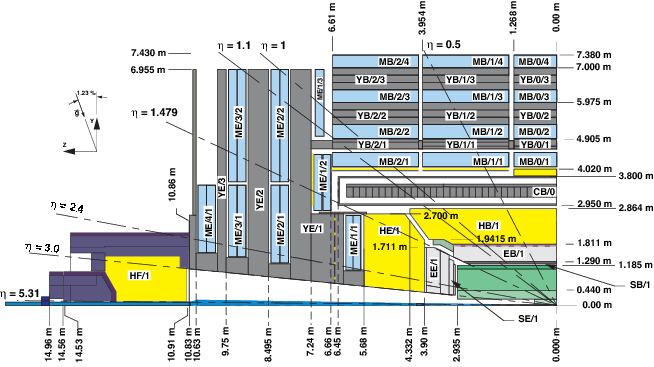
\includegraphics[height= 0.6\textwidth, width=0.8\textwidth]{THESISPLOTS/CMS_Int_View.png}} 
\captionof{figure}{Cross section view showing the coverage range of CMS sub-detectors and their longitudinal distance from the IP.}
\label{fig:cmslview}
\end{center}
\end{minipage}
%\clearpage

\vspace{5mm}
\begin{minipage}{0.99\textwidth} 
\begin{center}\label{CMS-SUBD}
\mbox{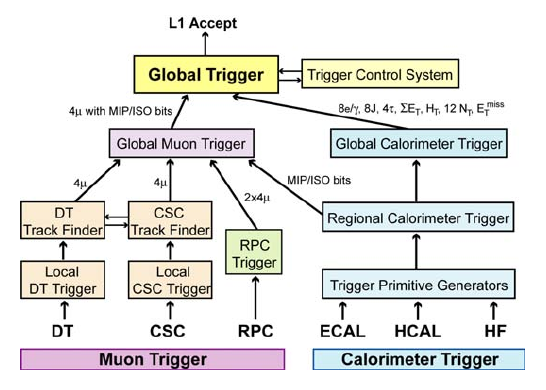
\includegraphics[height= 0.6\textwidth, width=0.8\textwidth]{THESISPLOTS/Level-1-Trigger-Architecture.png}}
\captionof{figure}{Level-1 trigger architecture of CMS.}
\label{fig:l1trigger}
\end{center}
\end{minipage}

\vspace{5mm}

\afterpage{ %
    \clearpage% Flush earlier floats (otherwise order might not be correct)
   %% \thispagestyle{empty}% empty page style (?)
  \begin{landscape}% Landscape page
\begin{minipage}{0.99\textwidth} 
\begin{center}
 %\setlength{\abovecaptionskip}{0pt}
  %\setlength{\belowcaptionskip}{10pt}
 % \topcaption{GMSB,GGM Phenomenology and Relevant final states}
  \begin{tabular}{l|l|p{3.2cm}|p{3.9cm}}
 % \hline \hline
  \multicolumn{4}{c}{\bfseries{CMS Detector Performance 2012}} \\
  \toprule
  \bfseries{Subdetector} & \bfseries{Quantity} & \bfseries{Resolution} & \bfseries{Uses}  \\
   \hline \hline
 Tracker   & Momentum[GeV/c]  & $\sigma_{T}/p_{T} \approx 1.5\times 10^{-4}p_{T} + 0.005$ & \mbox{Silicon Pixels and Strips} \\ 
  \hline
  ECAL   & Energy[GeV] & $\sigma/E \approx 3\% /E + 0.003$ & $\pb$ Crystals \\
   ECAL  & Time[ns] & $\sigma(\Delta t)= \frac{N}{A_{eff}/\sigma_{n}}\oplus\sqrt{2}\bar{C} $ & $\pb$ Crystals \\
  \hline
  HCAL & Energy[GeV] & $\sigma/E \approx 100\% /E + 0.05$ & Brass + Scintilator\\
  \hline
  Muon Chambers & Momentum[GeV/c] & $\sigma_{T}/p_{T} \approx$ 1\%  \@ 50 GeV to  10\% \@ 1 \TeV & inner tracker + Muon Systems \\
  \hline
  Magnetic field & B-field strength[T] & 3.8~T + 2~T & Solenoid + Return Yoke\\
  \hline
  Triggers  & On/Off-line & Levels &\mbox{L1(On-line)} +\mbox{HLT(Off-line)}(L2+L3) \\
  \hline
   \bottomrule
  \end{tabular}
  \captionof{table}{CMS detector performance for LHC RUN 1 \cite{CMSTDR2}. }
 \label{tab:tableCMS}
 \end{center}
\end{minipage}
\end{landscape}
 \clearpage% Flush page
}
%%%%%%%%%%%%%%%%%%%%%%%%%%%%%%%%%%%%%%%%%%%%%%%%%%%%%%%%%%%%%%%%%%%%%%%%%%%%%%%%
\label{Collider_And_Detector_chapter}
%%%%%%%%%%%%%%%%%%%%%%%%%%%%%%%%%%%%%%%%%%%%%%%%%%%%%%%%%%%%%%%%%%%%%%%%%%%%%%%%%
% Due to the large amount of data, such analysis are performed using clusters of computers geographically connected to each other in a virtual computing environment called the LHC Computing Grid~(LCG) to which the CMS is a member. This data is made available to 7 primary and later to secondary tier centres consisting of national research laboratories and universities around the world using a data transport system term Physics Experiment Data Export~(PhEDEx).

%%%%%%%%%%%%%%%%%%%%%%%%%%%%%%%%%%%%%%%%%%%%%%%%%%%%%%%%%%%%%%%%%%%%%%%%%%%%%%%%
%ranging from A Toroidal LHC Apparatus~(ATLAS) and
%both non-fixed target detectors, A Large Ion Collider Experiment~(ALICE) for colliding heavy ions and finally Large Hadron Collider beauty~(LHCb), a fixed target experiment for investigating the properties of B-Hadrons.
% We  give a full description of the important parts of the LHC in the following subsections, detail discussion of other interesting parts can be found here \cite{LHC}.
%There are three main steps prior to colliding protons or ions at the LHC.  The first is ramping up the energy of the beams followed by squeezing the beams at interaction points( CMS or ATLAS) and finally remove the separator bumps that are formed by local corrector magnets.

%\newline
%Another advantage is that, in circular colliders, like the LHC, the synchrotron radiation~(is inversely proportional to the mass of the circulating charge particle to the fourth power and contributes to the loss in energy by the circulating particle) from the  accelerating  proton is not significant, since the proton's mass is  about $0.938$\GeV, and its been accelerated to about 7\TeV. On the other hand if the accelerating particle were an electron, whose mass is about $0.000511$\GeV, then the energy loss due to synchrotron radiation will be very significant and one would require to continuously add energy after each turn to maintain the electron beam energy to a stable value. 
%However, since  more. Thus protons are preferred to electrons for a circular collider.
%Then again, the debris of particles produced when electrons collide is much less compared to that of protons making analysis in a hadron collider very challenging. 

%where the luminosity $\mathscr{L}$ is related to the total integrated luminosity(delivered luminosity over time) $\mathrm{L} = \int \mathscr{L}dt$ and is defined in terms of accelerator(assuming round beams and equal values of beta function) parameters as:

%\begin{equation}\label{eq:lumi}
%\mathscr{L} = \frac{1}{4\pi}\cdot\left(f_{rev}\mathit{n}_{b}\mathit{N}_{b}\right)\cdot\frac{\mathit{N}_{b}}{\varepsilon_{N}}\cdot \frac{\gamma}{\beta^{\ast}}\cdot \mathscr{R}(\theta_{c},\varepsilon,\beta^{\ast},\sigma_{z} )
%\end{equation}

%where $\mathit{N}_{b}$ is the number of particles per bunch, $\mathit{n}_{b}$ is the number of bunches, $f_{rev}$ is the revolutionary frequency, $\gamma = E/m_{p}$ is the relativistic factor, $\varepsilon_{N}$ is the normalised beam emittance which along with $\beta^{\ast}$, the value of the amplitude or beta function at interaction point, determines the size of the beam. $\mathscr{R}$ is the geometrical reduction factor arising from the fact that the beams to not collide head-on but at a non-zero angle called the crossing angle or \textit{"Piwinski angle"}( $\phi \equiv \frac{\theta_{c}\sigma_{z}}{2\sigma_{x}}$). This effect is known as the \textit{hour-glass effect}.
%From the above definition \ref{eq:lumi}, it is evident that keeping the emittance (meaning particles in beam are confined to a small distance and have nearly the same momentum ) means the likelihood of particle interaction will be greater and thus higher luminosity. However this is often not easy to archive as increasing the beam energy means reducing the beam emittance. The normalized emittance $\varepsilon_{N}$ is often used as its dependence on beam energy is a squared root dependence.
%In the same way, lower beta values implies the width of beam is narrower or properly \textit{"squeezed"} at interaction point resulting to an increase in number of collisions hence higher luminosity.
%This squeezing of depends on the quadruple magnet configuration and powering. 
%In addition to low beam emittance and lowest value of beta function at interaction point($\beta^{\ast}$), one can also archive higher luminosity by using high population bunches($\mathit{N}_{b}$) and collide them at high frequency.
%\%paragraph*{Luminosity Measurement}
%\par
%Obviously using equation \ref{eq:lumi} to determine the instantaneous and integrated luminosity would involve a lot of uncertainty in the measurements of about 20-30\%, as there are so many parameters whose value need to be measured precisely in a normal LHC operation. Rather specialised LHC runs known as \textit{"Van der Meer Scans"}\cite{lhclumi} are used to calibrate specialized equipments used for determining luminosity.
%The method employed by CMS(using TOTEM) is to use the total proton-proton~(\textit{p-p} cross section. 
%The method employed by CMS is using the Hadronic Foward~(HF) calorimeter to make luminosity measurements.
%Using production rates or cross sections of well and precisely calculable processes and rewriting \ref{eq:lumi} as:
%\begin{equation}\label{eq:LInt}
% \mathscr{L} \equiv \frac{Rate_{tot}}{\sigma_{tot}}    = \frac{\mu \mathit{n}_{b} f_{rev}}{\sigma_{tot}} 
%\end{equation}
%where $\mu = \left\langle \mathit{N}_{tot}/ \mathit{n}_{b} \right\rangle $ is the \textit{average number of interactions per bunch crossing}.

  
%of well understood and calculable processes such as the production of $\mathrm{W}$ and $\mathrm{Z}$ bosons or di-leptons via  two photon exchange. 
%\subsection{Superconducting Electromagnets}
%The LHC design and operation uses a total of 9593 powerful magnets of different types for different purposes. Since there are two beams of protons running in clock-wise and anti-clock wise directions, the LHC uses an ingenious technique design  of the magnetic field in every dipole magnet generates a vector field $\mathbb{B}$ in each pipe pointing in opposite direction to that of the other but both always perpendicular to the beam directions. The Lorentz or magnetic force acting on the protons in both pipes always point towards the center thus keeping the beams in circular motion. In circular accelerators as the LHC and its smaller synchrotron rings, given the accelerator radius,$R$, the beam energy $p$ is determined by the strength $\mathbf{B}$ of the magnetic field. This can be easily understood using the Lorentz force  such that $\displaystyle{p[TeV] = 0.3\mathbf{B}[T]\cdot R[km] }$.
%The LHC is is a 26.659~km in circumference machine using powerful dipole magnets with magnetic field strength of about 8.33~Tesla(T) are 7~TeV to keep the protons circulating in their curved path or orbits. The LHC operates using superfluid helium for heat transport at 1.4~K(-271.3~$^{\circ}C$)  temperature to prevent these near 1232 dipole magnets, 858 quadruple and 6208 correcting magnets from overheating due to the energy stored in these magnets. Conventional magnetics aren't convenient for modern particle accelerators with high center of mass energy for both performance and economic reason. Rather, superconducting magnets made with modern technology using  niobium-tantanium~(Nb-Ti) filaments strands or cables are used to provide the high magnetic field required. 
%These magnetics provide a magnetic field strength of about 8.33~T and are kept at about 1.4K in temperature during LHC operation.

%Quadrupole electromagnet and correcting magnets are  used to keep the particles in the beam and archive the required focus and de-focusing needed. At interaction point, the quadrupole magnets are held symmetrically around the beam pipe to help squeeze the proton beams to very low values of beta function thus ensuring that many particle collisions as possible necessary for higher luminosity.


%\subsection{Timing}
%The Large Hadron Collider (LHC) is designed to collide proton-proton (pp) bunches every  24.95~ns at designed luminosity. This means, the distance between each proton bunch is about 7.5~m compared to the nearly 100~m of optical fibre length which is required to transport readout information from the very front end electronics on the detectors to the back end  electronics at Point 5 for processing.
%It is therefore imperative to have a data synchronisation system for the trigger and readout systems of the LHC experiments in order that events from every proton-proton collision are properly assigned to the particular bunch crossing ~(BX) which produced them.
%The LHC is equipped with a Timing, Trigger and Control~(TTC) system with a bunch clock frequency of 40.07897~MHz whose function is to distribute synchronized LHC time to all the detectors including CMS.
%Timing synchronisation in the LHC is achieved using a Beam Synchronous Timing ~(BST) system which distributes timing using the LHC revolution frequency(at 11.246~kHz) or LHC orbit  and the RF bunch crossing frequency(40.07897~MHz at 7~\TeV). 
%Thus, the LHC fast timing signals from the RF generators  of the machine and orbit signals are distributed from the Prevessin Control Room~(PCR) through single-mode optical fibers(about 10.1~km in length for CMS) to all LHC experiments,  test beam areas, beam instrumentation around the ring and the SPS transfer lines.  At CMS counting room, the LHC clock and orbit signals  are recovered in the TTC Machine Interface crate~(TTCmi) and later distributed to the Trigger Control and sub-detector master TTC crates. All Level1~(L1) trigger and Data Acquisition~(DAQ) pipelines are driven with a 24.95~ns cycle clock locked to the LHC machine clock. The phase difference between the LHC 40~MHz clock and the arrival of detector signals from collision to the front-end electronics must be determined and adjusted for and monitored. The determination and assignment of pulses to bunch crossings depends critically on this initial clock phase adjustments and stability. This amplitude or pattern(also known as trigger primitives) for each trigger and bunch crossing is transmitted to the regional trigger logic in digital form every crossing and is synchronised with the LHC clock. Each trigger primitive digital data is then assigned to clock cycle in a process known as bunch crossing assignment. a   Detail expert description of LHC unified timing distribution system can be found here \cite{LHCT, LHCT1, LHCT2, LHCT3}.
%This means that there is the possibility of producing a LL particle when two protons collide every 25~ns.
%Thus it becomes a serious challenge  for triggering, data acquisition and associating the correct emerging particle to
%the correct bunch crossing (BX).
 %This is even more challenging for LL particles produced with low velocity since
%by design and read-out, with the time separation of 25~ns between BXs,
%Particles produced from LHC are assumed to be travelling at the speed of light (c = 299 792 458~m$s^{-1}$).
%Thus, such light speed particles will travel a distance of $\approx 7.5$~m.
%This leads to the possibility of having about 3 BXs  simultaneously contained in the Compact Muon Solenoid~(CMS) detector.
%As a result, LL particles produced with slower velocity might cause triggers to assigned particles to the wrong BX and so reduced the trigger
%efficiency for LL particles. An interesting study has been done by the another multi-purpose detector at CERN, ATLAS
%which looked at LL particle with different velocities~ $\beta$ and showed that it is important to enlarge triggering windows so as to increase
%triggering efficiencies for low velocity particles

%\subsection{Tracker}
%Particles produced from proton-proton collision traverse the tracker sub-detector first. The job of the tracker is to measure the trajectory of charged particles, which are curved because of the magnetic filed produced by the magnetic coils. By measuring the curvature of these particle, the particle's momentum can be measured and its charge determined. The tracker is a silicon based detector and thus operates under the concept of ionization. It occupies a volume of 2.4~m in diameter and 5.4~m in length, consisting of pixel and strip sections geometrically arrange in cylindrical layers of barrel and disc-shaped endcaps, enclosed within the calorimeters. These sub-detectors all sit inside the 6~m in diameter solenoid magnet operating at 3.8~T. Figure \eqref{fig:CMSTRAK} depicts a schematic picture of the tracker with three barrel layers covering a region of radius from 4~cm to 15~cm in radius and two endcap discs within 49~cm on either side of the collision point along the $z$ axis; ten barrels layers  and twelve endcap disks per side of silicon strip detectors covering a region with radius from 15 to 110~cm and within 280~cm on either side of the LHC beam axis. The total tracker acceptance region in pseudo-rapidity is $|\eta| < 2.5$. The pixel detector is used for identifying the primary and secondary vertices of particles while the inner tracker of strip detector is for tracker reconstruction. 
%\begin{center}\label{CMSTRAK}
%\centering
%\mbox{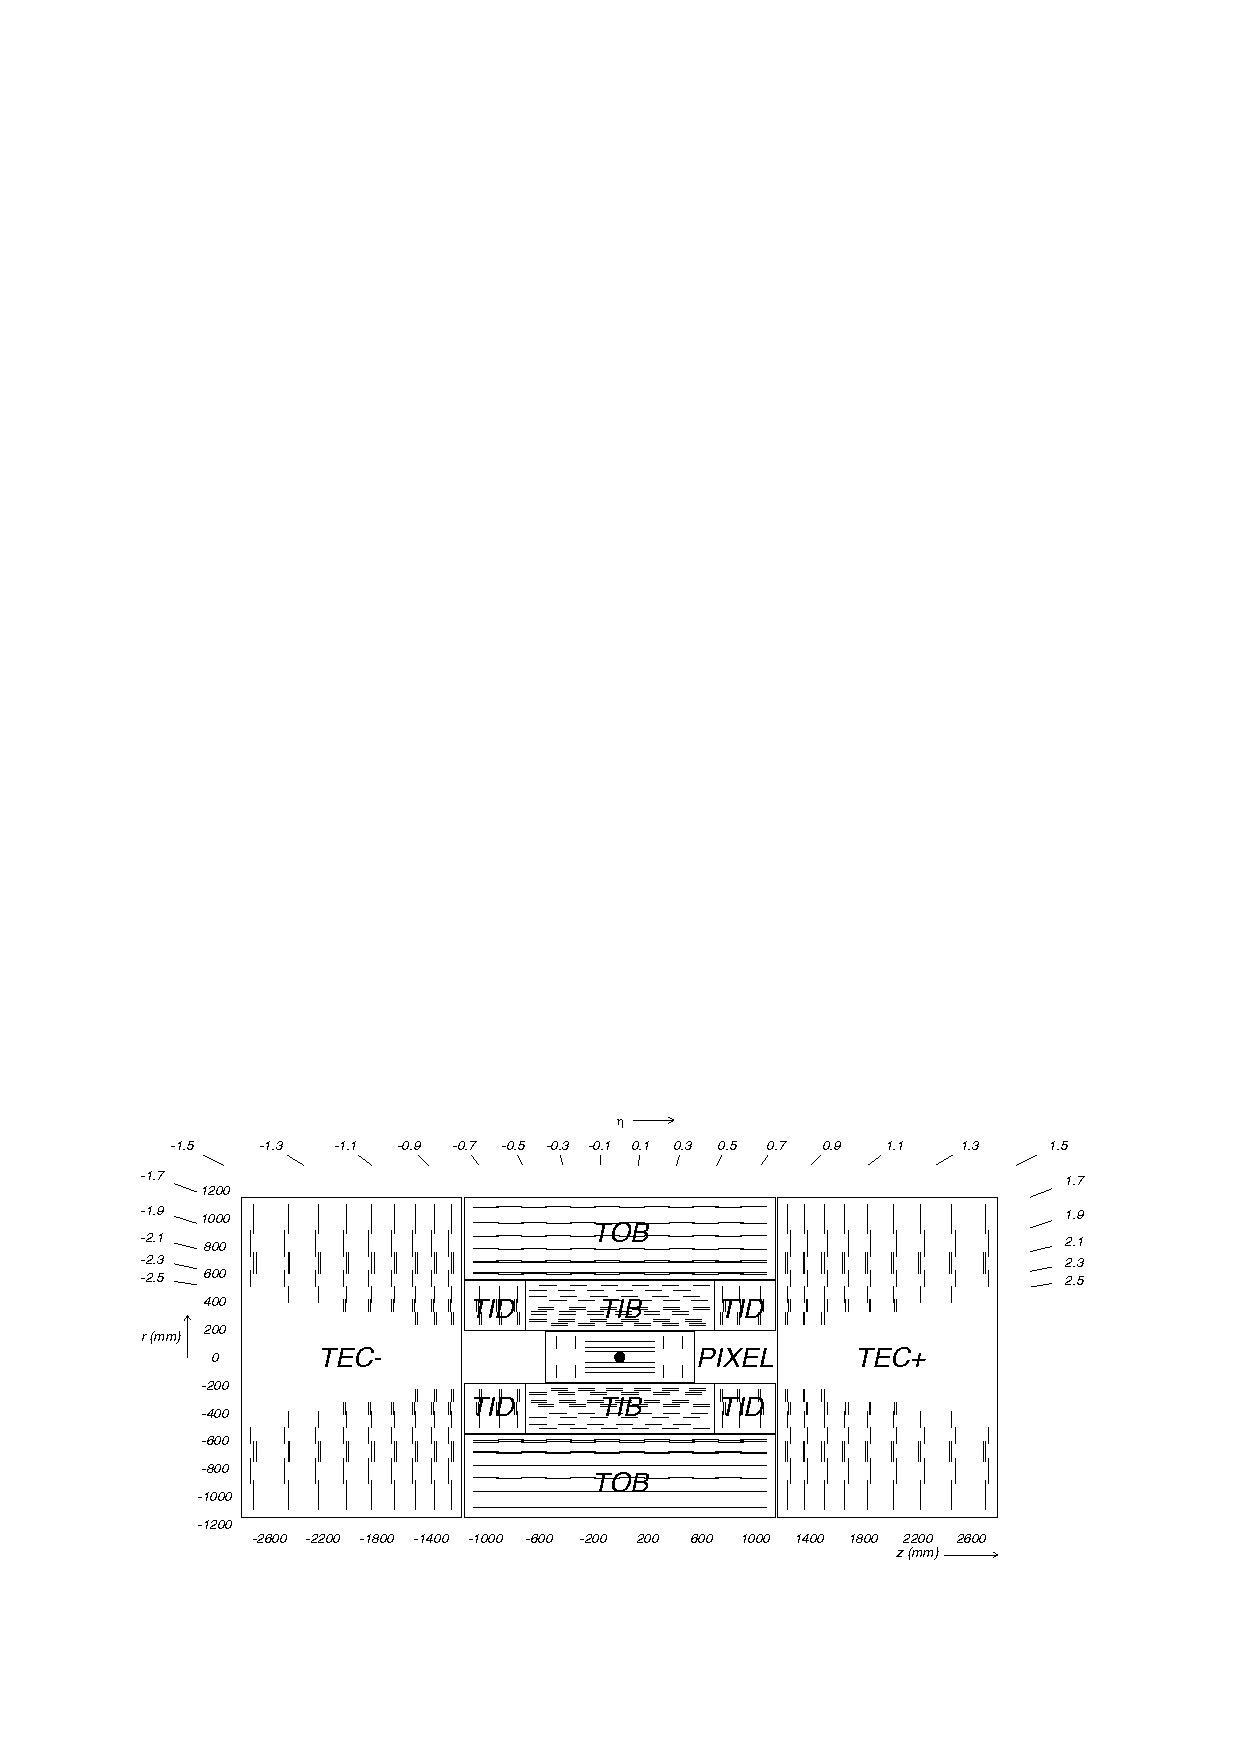
\includegraphics[scale=0.6]{THESISPLOTS/Tracker.pdf}} 
%\captionof{figure}{Schematic diagram of CMS Tracker showing the silicon pixel detector region~(inner closer to LHC beam) and silicon strip reigion~(outer).}
%\label{fig:CMSTRAK}
%\end{center}
%\subsubsection{Pixel}
%The pixel vertex detector occupies the inner most region, very closed to the interaction region. Providing high-resolution and three-dimensional patterns of space points using silicon pads as pixels, the primary vertex and secondary vertices arising from the decay of heavy and relatively long-lived particles such as B-mesons containing b-quarks can be identified. This is also known as impact parameter measurements. The pixel covering a region of pseudo-rapidity $|\eta| < 2.4$ compliments the track finding by providing additional space points to seeding hits in the inner tracker.  Each pixel has a size of $100\times150$~$\mu m^2$ 
%covering a total area of $\approx 1~m^{2}$ and there are 66 million pixels read out by 16000 readout chips on the silicon sensors. The pixel is organised in three 53~cm long barrel layers~(Pixel Barrel=PXB), positioned at radii  of 4.4, 7.3 and 10.2~cm and two disks each per side (Pixel Forward=PXF), placed at $\pm 34.5$~cm and $\pm46.5$~cm from the interaction point and covering a radii between 6 and 15~cm. This guarantees each charged particle track crosses at least two layers of pixels.
%This arrangement ensures that the pixel detector provides  precise tracking points in the $ r-\phi$ and $z$ responsible for small impact parameter resolution of about $\sim 15~\mu m$. Small impact parameter resolution is important for precise secondary vertex  reconstruction and position resolution crucial in the identification of objects produced with displaced vertices with life-time of  about $\tau \approx 10^{-12}~s$ like mesons such as $B^{0,{\pm}}$, $D^{0,{\pm}}$, $\tau^{\pm}$, which may travel a distinguishable distance (c$\tau$ $\approx 100~\mu$m before decaying. Because of very high radiation dose of about 100~Mrad absorbed by the pixel detector, there is currently upgrade of the complete pixel detector in preparation of LHC Run 2.

%\subsubsection{Silicon Strip Tracker}
%CMS silicon inner tracker surrounding the pixel detector allows for the tracks of promptly produced charged particles with $\PT = 100GeV/c$ to be reconstructed with a resolution in the transverse momentum \PT  of about $\sim 1.5\,\%$. High momentum particles are less curved by the magnetic field than low momentum particles. Therefore, the tracker works complimentary with the calorimeter and muon detectors to ensure improve momentum resolution at all particle energies.
%The silicon micro strip tracker covers a tracking volume up to radius of 1.2~m with a length of 5.6~m. It is organised in three parts: The inner tracker with four barrel layers (Tracker Inner Barrel=TIB) and three disks per endcap~(Tracker Inner Disks=TID), 6 outer barrel layers~(Tracker Outer Barrel=TOB) closed by 9 wheels on both sides.~(Tracker EndCap=TEC). 
%The silicon strip is made of 15148 silicon microstrip detector modules. Each module has a set of sensors. It occupies an active area of $200~m^{2}$ providing a coverage in pseudo-rapidity up to
% $|\eta| < 2.5 $.
% The TIB/TID delivers up to 4 $r-\phi$ measurements on a trajectory using 320~$\mu$m thick silicon micro strip sensors arranged  parallel to the beam direction in the barrel and radial on the disks. The strip pitch is 80~$\mu$m on layer 1 and 2 and 120~$\mu$m on layer 3 and 4 of the TIB, leading to a single point resolution of 23~$\mu$m and 35~$\mu$m, respectively. The TID also have varying pitches with both the TIB/TID enclosed by the TOB. The layering structure can be seen figure \eqref{CMSTRAK}. The nearly 9.6 million silicon strips provide a spatial resolution measured to be about $10~\mu$m for $r-\phi$ measurement and about $20~\mu$m for $z$ measurement necessary for particle trajectory reconstruction.
%The combined pixel and micro strip modules allows for nearly 75 million readout electronic channels in the tracker.


%%%The bunch structure is archived by  breaking a continuous proton beam into pulsed beam of separate bunches using an electromagnetic field  with oscillating frequency of 400~MHz(LHC ring) in the SPS and LHC RF cavity. Thus each bunch is in an RF bucket. 
 % with where each RF bucket has an energy against time profile as can be seen in figure below.
 %the rise/fall times at the SPS/LHC injection and ejection and to abort kickers magnets during
 %There is the possibility that ghost/satellite - ghost/satellite and ghost - Beam1/Beam2 collisions will happen generating events at the CMS detector. This is a major background in the search for delayed photons or objects in general as these collisions can occur \textit{in-time}(Beam1- Beam2) collisions or \textit{out-of-time} collisions. It is thus imperative to be able to quantify this contributions in any search analysis. We will show in future studies we have performs to both \textit{"guestimate"} and quantify these contributions in our search analysis.
 
 %\subsection{Particle Detection}
%Particle types that are identified using the CMS detector include electrons, photons, hadrons, muons, neutrinos and other weakly interacting particles. These particles depending on their charge, nature of interaction and lifetime can be identified either using some or all the sub-detectors of the CMS detector.
%The figure \ref{fig:cmsSLICE} show a  transverse slice of the CMS detectors with tracks in the tracker and muon sub-detectors and calorimeter energy deposit showing how different particles interact with the material in different sub-detectors thus ensuring their unique identification and reconstruction in the detector.
%\begin{center}
%\centering
%\mbox{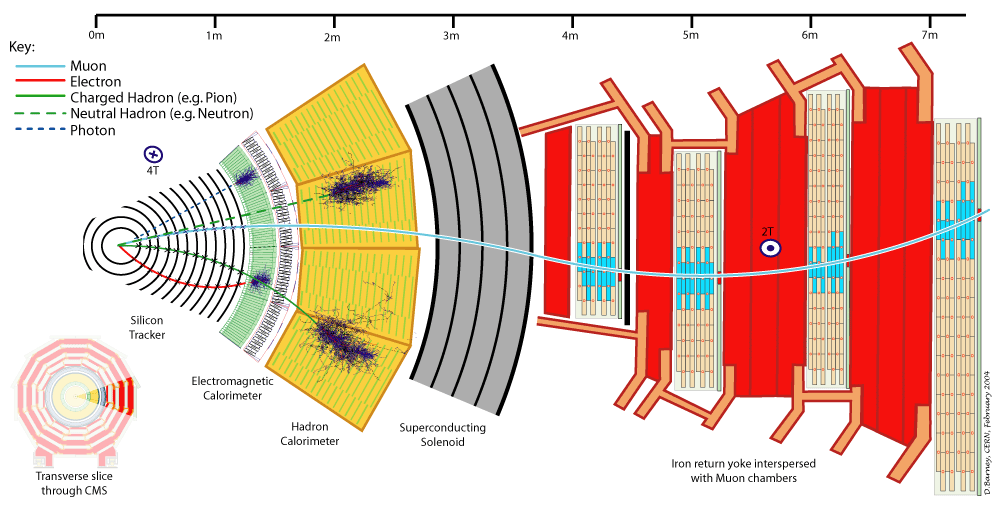
\includegraphics[scale=0.4]{THESISPLOTS/CMS_Slice.png}} 
%\captionof{figure}{Transverse slice of the CMS detector showing how different types of particles interact and hence identified using this detector.}
%\label{fig:cmsSLICE}
%\end{center}